\documentclass[12pt,portrait]{article}

\usepackage[a4paper,margin=1in]{geometry}
\usepackage{amsmath,amssymb}
\usepackage{booktabs}
\usepackage{multirow}
\usepackage{graphicx}
\usepackage{hyperref}
\usepackage{tcolorbox}
\usepackage{algorithm2e}
\usepackage{tikz}
\usepackage{forest}
\usepackage{array}
\usepackage{longtable}
\usepackage{enumitem}
\usepackage{microtype}
\usepackage{changepage}

\hypersetup{
    colorlinks=true,
    linkcolor=blue,
    urlcolor=cyan,
    pdftitle={Zero-Knowledge Algorithmic Playbook},
}

\newtcolorbox{warningbox}[1][]{colback=red!5!white,colframe=red!75!black,fonttitle=\bfseries,title=#1}
\newtcolorbox{rulebox}[1][]{colback=blue!5!white,colframe=blue!75!black,fonttitle=\bfseries,title=#1}
\newtcolorbox{examplebox}[1][]{colback=green!5!white,colframe=green!50!black,fonttitle=\bfseries,title=#1}

\begin{document}

\title{\Huge \textbf{Zero-Knowledge Algorithmic Playbook}\\[8pt]
\large DSA 61CSE108 -- Complete Exam Survival Guide}
\author{}
\date{}
\maketitle

\tableofcontents
\newpage

%%%%%%%%%%%%%%%%%%%%%%%%%%%%%%%%%%%%%%%%%%%%%%%%%%%%%%%%%%%%%%%%%%%%%%%%%%%%%%%
%%  SECTION 0: PROBLEM IDENTIFICATION INDEX
%%%%%%%%%%%%%%%%%%%%%%%%%%%%%%%%%%%%%%%%%%%%%%%%%%%%%%%%%%%%%%%%%%%%%%%%%%%%%%%

\section{The Problem Identification Index (Diagnostic Table)}

\begin{warningbox}[HOW TO USE THIS TABLE]
When you read an exam question, find the key phrase in the left column. The middle column tells you exactly which algorithm or data structure to use. The right column tells you which section of this playbook to open. Do not guess -- match the phrase.
\end{warningbox}

{\small
\begin{longtable}{p{4.2cm}|p{4.5cm}|p{4.5cm}}
\toprule
\textbf{Common Exam Phrasing} & \textbf{Algorithm / Data Structure} & \textbf{Playbook Section} \\
\midrule
\endhead
\bottomrule
\endfoot
``What is the time complexity?'' / ``Prove $f(n)=O(g(n))$'' / ``Find witness pair $c, n_0$'' & Asymptotic Limit Analysis ($O, \Omega, \Theta, o, \omega$) & \S\ref{sec:complexity} \\
\midrule
``Find the shortest route'' / ``Compute shortest paths from source'' (with edge weights) & Dijkstra's Algorithm & \S\ref{sec:dijkstra} \\
\midrule
``Find minimum spanning tree'' / ``Connect all nodes with minimum cost'' & Prim's or Kruskal's Algorithm & \S\ref{sec:mst} \\
\midrule
``Process in order of priority'' / ``Always remove the highest priority item'' & Priority Queue (Max-Heap) & \S\ref{sec:heap} \\
\midrule
``Evaluate this expression'' / ``Convert infix to postfix'' & Shunting-Yard / Postfix Evaluation (Stack) & \S\ref{sec:shunting} \\
\midrule
``Balance factors exceeding $\pm 1$'' / ``Restore AVL property'' & AVL Rotations (LL, RR, LR, RL) & \S\ref{sec:avl} \\
\midrule
``Delete a node with two children'' / ``Replace with inorder successor'' & BST Deletion + AVL Rebalancing & \S\ref{sec:avl_delete} \\
\midrule
``Given preorder and inorder, reconstruct the tree'' & Tree Reconstruction from Traversals & \S\ref{sec:tree_reconstruct} \\
\midrule
``Find LCS'' / ``Longest Common Subsequence'' & Dynamic Programming -- LCS & \S\ref{sec:lcs} \\
\midrule
``Optimal parenthesization'' / ``Matrix-chain multiplication'' & Dynamic Programming -- Matrix Chain & \S\ref{sec:mcm} \\
\midrule
``Maximize value with weight limit'' / ``0-1 Knapsack'' & Dynamic Programming -- 0-1 Knapsack & \S\ref{sec:knapsack} \\
\midrule
``Sort in ascending order'' / ``Apply QuickSort with median-of-three'' & Sorting Algorithms (Selection, Insertion, Heap, Merge, Quick, Radix) & \S\ref{sec:sorting} \\
\midrule
``Search a sorted array'' / ``Binary search on descending array'' & Binary Search & \S\ref{sec:binary_search} \\
\midrule
``Insert with collisions'' / ``Linear/Quadratic/Double probing'' & Hash Table Collision Resolution & \S\ref{sec:hashing} \\
\midrule
``Find middle node of linked list without extra memory'' & Slow/Fast Pointer Technique & \S\ref{sec:linkedlist} \\
\midrule
``Check if graph is connected'' / ``Count connected components'' & BFS / DFS Graph Traversal & \S\ref{sec:graph_traversal} \\
\bottomrule
\end{longtable}
}

\newpage

%%%%%%%%%%%%%%%%%%%%%%%%%%%%%%%%%%%%%%%%%%%%%%%%%%%%%%%%%%%%%%%%%%%%%%%%%%%%%%%
%%  SECTION 1: COMPLEXITY ANALYSIS COOKBOOK
%%%%%%%%%%%%%%%%%%%%%%%%%%%%%%%%%%%%%%%%%%%%%%%%%%%%%%%%%%%%%%%%%%%%%%%%%%%%%%%

\section{Complexity Analysis Cookbook}
\label{sec:complexity}

\subsection{The Five Asymptotic Notations: What They Actually Mean}

\begin{rulebox}[Plain-English Definitions]
\begin{itemize}[leftmargin=*]
    \item \textbf{Big-Oh $O(g)$}: ``My function $f$ grows \textbf{no faster than} $g$, once you ignore constants and small inputs.'' Think: $f$ is \textbf{at most} proportional to $g$. This is the \textbf{upper bound}.
    \item \textbf{Big-Omega $\Omega(g)$}: ``My function $f$ grows \textbf{at least as fast as} $g$, once you ignore constants and small inputs.'' Think: $f$ is \textbf{at least} proportional to $g$. This is the \textbf{lower bound}.
    \item \textbf{Big-Theta $\Theta(g)$}: ``My function $f$ grows \textbf{exactly like} $g$, once you ignore constants and small inputs.'' Think: $f$ and $g$ are \textbf{of the same order}. This is the \textbf{tight bound}.
    \item \textbf{Little-Oh $o(g)$}: ``My function $f$ grows \textbf{strictly slower than} $g$, even if you multiply $g$ by a tiny constant.'' Use the limit test: $\lim_{n\to\infty} f/g = 0$.
    \item \textbf{Little-Omega $\omega(g)$}: ``My function $f$ grows \textbf{strictly faster than} $g$, even if you multiply $g$ by a huge constant.'' Use the limit test: $\lim_{n\to\infty} f/g = \infty$.
\end{itemize}
\end{rulebox}

\subsection{The Limit Rule: Your One-Line Classifier}

Compute $L = \displaystyle\lim_{n \to \infty} \dfrac{f(n)}{g(n)}$. Then:

\begin{center}
\begin{tabular}{c|c|c|c|c|c}
\toprule
$L$ & $f = o(g)$ & $f = \Omega(g)$ & $f = \Theta(g)$ & $f = O(g)$ & $f = \omega(g)$ \\
\midrule
$0$ & \checkmark & & & \checkmark & \\
$(0,\infty)$ & & \checkmark & \checkmark & \checkmark & \\
$\infty$ & & \checkmark & & & \checkmark \\
\bottomrule
\end{tabular}
\end{center}

\begin{examplebox}[How to read this table]
If $\lim_{n\to\infty} \frac{n^2+3}{n^2} = 1$ (which is in $(0,\infty)$), then $n^2+3 = \Theta(n^2)$, $n^2+3 = O(n^2)$, AND $n^2+3 = \Omega(n^2)$.
\end{examplebox}

\subsection{Proving Big-Oh by Finding Witness Pairs $(c, n_0)$}

The definition says: $f(n) = O(g(n))$ if there exist positive constants $c$ and $n_0$ such that for ALL $n \geq n_0$, we have $f(n) \leq c \cdot g(n)$.

\textbf{The mechanical recipe:}
\begin{enumerate}[leftmargin=*]
    \item Expand $f(n)$ into individual terms.
    \item Bump up each term's power to match the power of $g(n)$. (For example, if $g(n)=n^2$, turn $2n$ into $2n^2$.)
    \item Sum up all the coefficients. That sum is your candidate $c$.
    \item Choose $n_0=1$ (almost always works for polynomials).
    \item Verify: for $n \geq n_0$, does $f(n) \leq c \cdot g(n)$ hold?
\end{enumerate}

\subsubsection{Fully Solved Example 1: Proving $n^2 + 2n + 5 = O(n^2)$}

\begin{rulebox}[Plain-English Logic Beside Math]
We want to show $n^2 + 2n + 5$ is eventually bounded above by some constant multiple of $n^2$. Since $n^2$ grows fastest, the other terms are ``cheap'' compared to $n^2$ when $n$ is large. We just need to over-approximate each smaller term as a term of the same degree as $g(n)$.

\textbf{Step 1 -- Set up the inequality:}
We need $c$ and $n_0$ such that for all $n \geq n_0$:
$$n^2 + 2n + 5 \leq c \cdot n^2$$

\textbf{Step 2 -- Over-approximate each term for $n \geq 1$:}
\begin{itemize}[leftmargin=*]
    \item $n^2$ is already the right form; it equals $1\cdot n^2$.
    \item $2n$: since $n \geq 1$, we know $n \leq n^2$, so $2n \leq 2n^2$.
    \item $5$: since $n \geq 1$, we know $1 \leq n^2$, so $5 \leq 5n^2$.
\end{itemize}

\textbf{Step 3 -- Sum the coefficients:}
$$n^2 + 2n + 5 \leq 1n^2 + 2n^2 + 5n^2 = 8n^2$$

\textbf{Step 4 -- Choose witness pair:}
$$c = 8, \quad n_0 = 1$$

\textbf{Step 5 -- Final verification:}
For all $n \geq 1$:
$$n^2 + 2n + 5 \leq 1n^2 + 2n^2 + 5n^2 = 8n^2$$
The inequality holds.
\end{rulebox}

\subsubsection{Fully Solved Example 2: Proving $3n + 10 = O(n)$}

\begin{rulebox}[Plain-English Logic Beside Math]
\textbf{Step 1 -- Set up:} Need $c, n_0$ such that $3n + 10 \leq c \cdot n$ for all $n \geq n_0$.

\textbf{Step 2 -- Over-approximate:} For $n \geq 1$:
\begin{itemize}[leftmargin=*]
    \item $3n$ is $3n$.
    \item $10 \leq 10n$ (since $n \geq 1$).
\end{itemize}
So: $3n + 10 \leq 3n + 10n = 13n$.

\textbf{Step 3 -- Witness pair:} $c = 13$, $n_0 = 1$.

\textbf{Verification:} For all $n \geq 1$, $3n + 10 \leq 13n$.
\end{rulebox}

\subsubsection{Fully Solved Example 3: Proving $5\log n + 7 = O(\log n)$}

\begin{rulebox}[Plain-English Logic Beside Math]
\textbf{Step 1 -- Set up:} Need $c, n_0$ such that $5\log n + 7 \leq c \cdot \log n$ for all $n \geq n_0$.

\textbf{Step 2 -- Over-approximate the constant:} For $n \geq 2$, we have $\log n \geq 1$, so $7 \leq 7\log n$.

Therefore: $5\log n + 7 \leq 5\log n + 7\log n = 12\log n$.

\textbf{Step 3 -- Witness pair:} $c = 12$, $n_0 = 2$.

\textbf{Verification:} For all $n \geq 2$, $5\log n + 7 \leq 12\log n$.
\end{rulebox}

\subsubsection{Fully Solved Example 4: Proving $n^2 + 100n\log n = O(n^2 \log n)$}

\begin{rulebox}[Plain-English Logic Beside Math]
\textbf{Step 1 -- Set up:} Need $c, n_0$ such that $n^2 + 100n\log n \leq c \cdot n^2\log n$ for all $n \geq n_0$.

\textbf{Step 2 -- Over-approximate both terms:} For $n \geq 2$, we have $\log n \geq 1$, so:
\begin{itemize}[leftmargin=*]
    \item $n^2 \leq n^2\log n$ (multiply by $\log n \geq 1$)
    \item $100n\log n \leq 100n^2\log n$ (multiply by $n \geq 1$)
\end{itemize}
Therefore: $n^2 + 100n\log n \leq n^2\log n + 100n^2\log n = 101n^2\log n$.

\textbf{Step 3 -- Witness pair:} $c = 101$, $n_0 = 2$.
\end{rulebox}

\subsection{Finding Witness Pairs for Big-Omega $\Omega$}

For $\Omega$, we need a LOWER bound: $f(n) \geq c \cdot g(n)$. The trick is to DROP positive terms to get a smaller expression, then divide.

\subsubsection{Fully Solved Example: Proving $n^2 + 2n + 5 = \Omega(n^2)$}

\begin{rulebox}[Plain-English Logic Beside Math]
\textbf{Step 1 -- Set up:} Need $c, n_0$ such that $n^2 + 2n + 5 \geq c \cdot n^2$ for all $n \geq n_0$.

\textbf{Step 2 -- Drop positive lower-order terms:} Since $2n \geq 0$ and $5 \geq 0$, we have:
$$n^2 + 2n + 5 \geq n^2 = 1 \cdot n^2$$

\textbf{Step 3 -- Witness pair:} $c = 1$, $n_0 = 1$.

\textbf{Verification:} For all $n \geq 1$, $n^2 + 2n + 5 \geq n^2$.
\end{rulebox}

\subsection{Finding Witness Pairs for Big-Theta $\Theta$}

Combine the $O$ and $\Omega$ witness pairs. You need both an upper bound constant $c_2$ and a lower bound constant $c_1$, plus a shared $n_0$.

\subsubsection{Fully Solved Example: Proving $n^2 + 2n + 5 = \Theta(n^2)$}

\begin{rulebox}[Plain-English Logic Beside Math]
From above:
\begin{itemize}[leftmargin=*]
    \item $O$ bound: $n^2 + 2n + 5 \leq 8n^2$ for $n \geq 1$. So $c_2 = 8$.
    \item $\Omega$ bound: $n^2 + 2n + 5 \geq 1n^2$ for $n \geq 1$. So $c_1 = 1$.
\end{itemize}
Combining: $1\cdot n^2 \leq n^2 + 2n + 5 \leq 8\cdot n^2$ for all $n \geq 1$.

Witness triple: $(c_1=1, c_2=8, n_0=1)$.
\end{rulebox}

\subsection{Growth Rate Hierarchy (Memorize This Order)}
\begin{center}
\begin{tcolorbox}[colback=yellow!10!white,colframe=yellow!50!black,title=Slowest $\to$ Fastest]
$$O(1) \;\subset\; O(\log n) \;\subset\; O(\sqrt{n}) \;\subset\; O(n) \;\subset\; O(n\log n) \;\subset\; O(n^2) \;\subset\; O(n^3) \;\subset\; O(2^n) \;\subset\; O(n!)$$
\end{tcolorbox}
\end{center}

\textbf{Key facts:} Any polynomial beats any logarithm. Any exponential beats any polynomial. $\log n! = \Theta(n\log n)$.

\subsection{Quick Limit Computation Shortcuts}

\begin{itemize}[leftmargin=*]
    \item $\displaystyle\lim_{n\to\infty}\frac{\log n}{n^c} = 0$ for any $c > 0$. (Logarithms lose to any positive power of $n$.)
    \item $\displaystyle\lim_{n\to\infty}\frac{n^a}{b^n} = 0$ for any $a > 0$, $b > 1$. (Polynomials lose to exponentials.)
    \item $\displaystyle\lim_{n\to\infty}\frac{n!}{n^n} = 0$ via Stirling: $n! \approx \sqrt{2\pi n}\,(n/e)^n$.
    \item For summing loops: $\sum_{i=1}^{n} i = \frac{n(n+1)}{2} = \Theta(n^2)$. $\sum_{i=1}^{n} i^2 = \Theta(n^3)$.
    \item Geometric series with $r<1$: $\sum_{i=0}^{\infty} r^i = \frac{1}{1-r}$. With $r=1/2$, sum $\approx 2$.
\end{itemize}

%%%%%%%%%%%%%%%%%%%%%%%%%%%%%%%%%%%%%%%%%%%%%%%%%%%%%%%%%%%%%%%%%%%%%%%%%%%%%%%
%%  SECTION 2: ALGORITHM EXECUTION TRACE PLAYBOOK
%%%%%%%%%%%%%%%%%%%%%%%%%%%%%%%%%%%%%%%%%%%%%%%%%%%%%%%%%%%%%%%%%%%%%%%%%%%%%%%
\section{Algorithm Execution Trace Playbook (Search \& Sort)}
\label{sec:sorting}

\subsection{Binary Search -- Step-by-Step Trace}
\label{sec:binary_search}

\begin{rulebox}[The Exact Conditional Logic for Binary Search]
\begin{enumerate}[leftmargin=*]
    \item Set $\text{left} = 0$, $\text{right} = n-1$, $\text{result} = -1$.
    \item While $\text{left} \leq \text{right}$:
    \begin{enumerate}
        \item Compute $\text{mid} = \lfloor(\text{left} + \text{right}) / 2\rfloor$.
        \item If $A[\text{mid}] = \text{target}$, set $\text{result} = \text{mid}$ and stop.
        \item If $\text{target} > A[\text{mid}]$, the target is in the RIGHT half. Set $\text{left} = \text{mid} + 1$. Cross out the entire left half (indices below mid).
        \item If $\text{target} < A[\text{mid}]$, the target is in the LEFT half. Set $\text{right} = \text{mid} - 1$. Cross out the entire right half (indices above mid).
    \end{enumerate}
    \item Return the result.
\end{enumerate}
\end{rulebox}

\subsubsection{Worked Trace: Search for 6 in sorted array $[1,2,3,5,6,7,9,19]$}

\begin{center}
\begin{tabular}{c|c|c|c|c|c}
\toprule
\textbf{Iteration} & \textbf{left} & \textbf{right} & \textbf{mid} & $A[\text{mid}]$ & \textbf{Decision} \\
\midrule
Start & 0 & 7 & -- & -- & -- \\
1 & 0 & 7 & $\lfloor(0+7)/2\rfloor = 3$ & $A[3]=5$ & $6 > 5$ $\to$ go RIGHT, left=4 \\
2 & 4 & 7 & $\lfloor(4+7)/2\rfloor = 5$ & $A[5]=7$ & $6 < 7$ $\to$ go LEFT, right=4 \\
3 & 4 & 4 & $\lfloor(4+4)/2\rfloor = 4$ & $A[4]=6$ & MATCH! Return 4 \\
\bottomrule
\end{tabular}
\end{center}

\subsubsection{Blank Template for Exam Use}

\begin{center}
\begin{tabular}{c|c|c|c|c|c}
\toprule
\textbf{Iteration} & \textbf{left} & \textbf{right} & \textbf{mid} & $A[\text{mid}]$ & \textbf{Decision} \\
\midrule
Start & & & -- & -- & -- \\
1 & & & & & \\
2 & & & & & \\
3 & & & & & \\
4 & & & & & \\
5 & & & & & \\
\bottomrule
\end{tabular}
\end{center}

\textbf{Key exam fact:} For a sorted array of 32 elements, the maximum number of comparisons to determine a missing key or find the last possible position is $\lceil\log_2 32\rceil = 6$. Each comparison cuts the remaining search space in half.

\subsection{Selection Sort -- Complete Trace}

\begin{rulebox}[Selection Sort Logic in Plain English]
\begin{enumerate}[leftmargin=*]
    \item Start at position $i=0$ (the leftmost unsorted position).
    \item Scan the entire unsorted portion ($A[i]$ through $A[n-1]$) to find the smallest element. Remember its index.
    \item Swap that smallest element with $A[i]$.
    \item Advance $i$ by 1. The portion $A[0..i-1]$ is now permanently sorted and will never be touched again.
    \item Repeat from Step 2 until $i = n-1$.
\end{enumerate}
\end{rulebox}

\subsubsection{Trace: Selection Sort on $[7,2,1,5,3,6,19,9]$}

\begin{center}
\begin{tabular}{c|c|c|l}
\toprule
\textbf{Pass $i$} & \textbf{Unsorted range} & \textbf{Min found} & \textbf{Array after swap} \\
\midrule
0 & $[7,2,1,5,3,6,19,9]$ & $A[2]=1$ & $[\mathbf{1},2,7,5,3,6,19,9]$ \\
1 & $[2,7,5,3,6,19,9]$ & $A[1]=2$ & $[1,\mathbf{2},7,5,3,6,19,9]$ \\
2 & $[7,5,3,6,19,9]$ & $A[4]=3$ & $[1,2,\mathbf{3},5,7,6,19,9]$ \\
3 & $[5,7,6,19,9]$ & $A[3]=5$ & $[1,2,3,\mathbf{5},7,6,19,9]$ \\
4 & $[7,6,19,9]$ & $A[5]=6$ & $[1,2,3,5,\mathbf{6},7,19,9]$ \\
5 & $[7,19,9]$ & $A[5]=7$ & $[1,2,3,5,6,\mathbf{7},19,9]$ \\
6 & $[19,9]$ & $A[7]=9$ & $[1,2,3,5,6,7,\mathbf{9},19]$ \\
7 & $[19]$ & $A[7]=19$ & $[1,2,3,5,6,7,9,\mathbf{19}]$ \\
\bottomrule
\end{tabular}
\end{center}

\subsubsection{Blank Selection Sort Template}

\begin{center}
\begin{tabular}{c|c|c|l}
\toprule
\textbf{Pass $i$} & \textbf{Unsorted range} & \textbf{Min found} & \textbf{Array after swap} \\
\midrule
0 & & & \\
1 & & & \\
2 & & & \\
3 & & & \\
4 & & & \\
5 & & & \\
6 & & & \\
7 & & & \\
\bottomrule
\end{tabular}
\end{center}

\subsection{Insertion Sort -- Complete Trace}

\begin{rulebox}[Insertion Sort Logic in Plain English]
Think of sorting playing cards in your hand:
\begin{enumerate}[leftmargin=*]
    \item Consider $A[0]$ as a sorted ``hand'' of 1 card.
    \item Take the next card $A[i]$ from the unsorted pile. Call it the ``key.''
    \item Look at the sorted hand from right to left. For each card in the hand that is BIGGER than the key, shift that card one position to the right.
    \item Stop shifting when you find a card $\leq$ the key (or you reach the left end).
    \item Insert the key into the empty slot you just created.
    \item Repeat from Step 2 for all remaining cards.
\end{enumerate}
\end{rulebox}

\subsubsection{Trace: Insertion Sort on $[7,2,1,5,3,6,19,9]$}

\begin{center}
\begin{tabular}{c|c|c|l}
\toprule
\textbf{$i$} & \textbf{key} & \textbf{Shifting action} & \textbf{Array after insertion} \\
\midrule
1 & 2 & $7>2$, shift 7 right; insert 2 at pos 0 & $[2,7,1,5,3,6,19,9]$ \\
2 & 1 & $7>1$ shift, $2>1$ shift; insert 1 at pos 0 & $[1,2,7,5,3,6,19,9]$ \\
3 & 5 & $7>5$ shift; $2\leq5$ stop; insert 5 at pos 2 & $[1,2,5,7,3,6,19,9]$ \\
4 & 3 & $7>3$ shift, $5>3$ shift, $2\leq3$ stop; insert 3 at pos 2 & $[1,2,3,5,7,6,19,9]$ \\
5 & 6 & $7>6$ shift, $5\leq6$ stop; insert 6 at pos 4 & $[1,2,3,5,6,7,19,9]$ \\
6 & 19 & $7\leq19$ stop; insert at pos 6 & $[1,2,3,5,6,7,19,9]$ \\
7 & 9 & $19>9$ shift, $7\leq9$ stop; insert 9 at pos 6 & $[1,2,3,5,6,7,9,19]$ \\
\bottomrule
\end{tabular}
\end{center}

\subsection{Heap Sort -- Complete Trace}
\label{sec:heap}

\begin{rulebox}[Three Heap Facts You Must Know]
\begin{enumerate}[leftmargin=*]
    \item A \textbf{max-heap} means: every parent is $\geq$ both its children. The root is always the largest element.
    \item For an array index $i$: left child is at $2i+1$, right child is at $2i+2$, parent is at $\lfloor(i-1)/2\rfloor$.
    \item Leaves occupy indices $\lfloor n/2\rfloor$ through $n-1$. Leaves are trivially valid heaps (they have no children to compare with).
\end{enumerate}
\end{rulebox}

\begin{center}
\begin{tikzpicture}[level distance=1.2cm,level 1/.style={sibling distance=3cm},level 2/.style={sibling distance=1.5cm},level 3/.style={sibling distance=1cm}]
\node {62}
    child {node {53}
        child {node {41}
            child {node {32}}
            child {node {12}}
        }
        child {node {49}
            child {node {30}}
            child[missing]
        }
    }
    child {node {14}
        child {node {3}}
        child {node {1}}
    };
\end{tikzpicture}
\end{center}

\textbf{Heap array representation:} $[62, 53, 14, 41, 49, 3, 1, 32, 12, 30]$

\subsubsection{Heap Sort: Two-Phase Process}

\begin{rulebox}[Phase 1: Build Max-Heap]
Starting from the last non-leaf node (index $\lfloor n/2\rfloor-1$), call Heapify on each node, moving upward to the root.

For array $[1, 30, 3, 12, 53, 62, 14, 32, 41, 49]$ with $n=10$:
\begin{itemize}[leftmargin=*]
    \item Last non-leaf: index $\lfloor 10/2\rfloor - 1 = 4$, value $A[4]=53$.
    \item Call Heapify on indices 4, 3, 2, 1, 0 in that order.
\end{itemize}
\end{rulebox}

\begin{rulebox}[Phase 2: Extract-Sort]
Repeat $n-1$ times:
\begin{enumerate}[leftmargin=*]
    \item Swap the root ($A[0]$, which is the maximum) with the last element of the current heap ($A[\text{heap\_size}-1]$).
    \item Decrease heap size by 1 (the last position now holds a sorted element).
    \item Call Heapify on the root (index 0) to restore the max-heap property.
\end{enumerate}
\end{rulebox}

\subsubsection{Heapify at a Single Node (Exact Algorithm)}

\begin{rulebox}[Heapify(A, n, i) Logic]
\begin{enumerate}[leftmargin=*]
    \item Set $\text{largest} = i$.
    \item Compute $\text{left} = 2i+1$, $\text{right} = 2i+2$.
    \item If $\text{left} < n$ AND $A[\text{left}] > A[\text{largest}]$, then set $\text{largest} = \text{left}$.
    \item If $\text{right} < n$ AND $A[\text{right}] > A[\text{largest}]$, then set $\text{largest} = \text{right}$.
    \item If $\text{largest} \neq i$: swap $A[i]$ with $A[\text{largest}]$, then recursively call Heapify on index $largest$ (the position where the smaller value ``sank'' to).
\end{enumerate}
\end{rulebox}

\subsection{Merge Sort -- Complete Trace}

\begin{rulebox}[Merge Sort Logic in Plain English]
\begin{enumerate}[leftmargin=*]
    \item \textbf{Divide:} If the subarray has 0 or 1 element, it is already sorted. Otherwise, split it into two halves at the midpoint.
    \item \textbf{Conquer:} Recursively sort the left half, then recursively sort the right half.
    \item \textbf{Combine:} Merge the two sorted halves by comparing the smallest remaining element of each half and picking the smaller one, copying into a temporary array, then copying back.
\end{enumerate}
\end{rulebox}

\subsubsection{Trace: Merge Sort on $[7,2,1,5,3,6,19,9]$}

\textbf{Divide phase (recursive splitting into halves):}
\begin{verbatim}
[7,2,1,5,3,6,19,9]
  -> [7,2,1,5]           [3,6,19,9]
    -> [7,2]   [1,5]       -> [3,6]   [19,9]
      -> [7] [2] [1] [5]     -> [3] [6] [19] [9]
\end{verbatim}

\textbf{Merge phase (bottom-up merging):}
\begin{verbatim}
Merge([7],[2]) -> [2,7]        Merge([1],[5]) -> [1,5]
Merge([3],[6]) -> [3,6]        Merge([19],[9]) -> [9,19]
Merge([2,7],[1,5]) -> [1,2,5,7]   Merge([3,6],[9,19]) -> [3,6,9,19]
Merge([1,2,5,7],[3,6,9,19]) -> [1,2,3,5,6,7,9,19]
\end{verbatim}

\subsubsection{How Merge Works, Element by Element (Merging $[2,7]$ and $[1,5]$)}

\begin{center}
\begin{tabular}{c|c|c|c|l}
\toprule
\textbf{Step} & \textbf{Left ptr} & \textbf{Right ptr} & \textbf{Compare} & \textbf{Temp array so far} \\
\midrule
1 & $A[0]=2$ & $A[0']=1$ & $1 < 2$, take 1 & $[1]$ \\
2 & $A[0]=2$ & $A[1']=5$ & $2 < 5$, take 2 & $[1,2]$ \\
3 & $A[1]=7$ & $A[1']=5$ & $5 < 7$, take 5 & $[1,2,5]$ \\
4 & $A[1]=7$ & -- & Left remaining & $[1,2,5,7]$ \\
\bottomrule
\end{tabular}
\end{center}

\subsection{Quick Sort -- Complete Trace}

\begin{rulebox}[Quick Sort Logic in Plain English]
\begin{enumerate}[leftmargin=*]
    \item \textbf{Choose pivot:} Pick the last element of the subarray as the pivot.
    \item \textbf{Partition:} Rearrange the subarray so that:
    \begin{itemize}[leftmargin=*]
        \item All elements $<$ pivot come before the pivot.
        \item All elements $\geq$ pivot come after the pivot.
        \item The pivot ends up in its final sorted position.
    \end{itemize}
    \item \textbf{Recurse:} Sort the left portion (indices before pivot), then sort the right portion (indices after pivot).
    \item Base case: a subarray with 0 or 1 element is already sorted.
\end{enumerate}
\end{rulebox}

\subsubsection{Partition Algorithm (Step-by-Step)}

Given $A[\text{low}..\text{high}]$ with $\text{pivot} = A[\text{high}]$:
\begin{enumerate}[leftmargin=*]
    \item Set $i = \text{low} - 1$ (this marks the boundary of the ``less than pivot'' region).
    \item Loop $j$ from $\text{low}$ to $\text{high}-1$:
    \begin{itemize}[leftmargin=*]
        \item If $A[j] < \text{pivot}$: increment $i$, then swap $A[i]$ with $A[j]$.
        \item If $A[j] \geq \text{pivot}$: do nothing, just advance $j$.
    \end{itemize}
    \item After the loop, swap $A[i+1]$ with $A[\text{high}]$ (this places the pivot in its correct position).
    \item Return $i+1$ as the pivot's final index.
\end{enumerate}

\subsubsection{Partition Trace: $[7,2,1,5,3,6,19,9]$, pivot = 9}

\begin{center}
\begin{tabular}{c|c|c|c|l}
\toprule
$j$ & $A[j]$ & $A[j] < 9$? & $i$ after & Array state \\
\midrule
0 & 7 & Yes & 0 & Swap(0,0): no change $[7,2,1,5,3,6,19,9]$ \\
1 & 2 & Yes & 1 & Swap(1,1): no change $[7,2,1,5,3,6,19,9]$ \\
2 & 1 & Yes & 2 & Swap(2,2): no change $[7,2,1,5,3,6,19,9]$ \\
3 & 5 & Yes & 3 & Swap(3,3): no change $[7,2,1,5,3,6,19,9]$ \\
4 & 3 & Yes & 4 & Swap(4,4): no change $[7,2,1,5,3,6,19,9]$ \\
5 & 6 & Yes & 5 & Swap(5,5): no change $[7,2,1,5,3,6,19,9]$ \\
6 & 19 & No & 5 & No swap \\
\bottomrule
\end{tabular}

\textbf{Final swap:} Swap $A[6]$ (pivot=9) with $A[6]$ (itself). Pivot at index 6. \\
\textbf{Result:} Left of index 6: $[7,2,1,5,3,6]$ (all $<9$), index 6: $[9]$, right: $[19]$.
\end{center}

\subsubsection{Median-of-Three Pivot Selection (Exam Technique)}

\begin{rulebox}[How to Pick Median-of-Three Pivot]
Given the array, look at three positions:
\begin{itemize}[leftmargin=*]
    \item \textbf{First element}: $A[\text{low}]$
    \item \textbf{Middle element}: $A[\text{mid}]$ where $\text{mid} = \lfloor(\text{low}+\text{high})/2\rfloor$
    \item \textbf{Last element}: $A[\text{high}]$
\end{itemize}
Take these three values, sort them, and select the MEDIAN (middle) value as the pivot. Then physically swap that median value with $A[\text{high}]$ so the usual last-element partition code works.

\textbf{Example:} For array $[1,30,3,12,53,62,14,32,41,49]$ with $n=10$:
\begin{itemize}[leftmargin=*]
    \item First: $A[0]=1$, Middle: $A[4]=53$, Last: $A[9]=49$
    \item Sorted: 1, 49, 53. Median = 49.
    \item Pivot = 49. Swap 49 with $A[9]$.
\end{itemize}
\end{rulebox}

\subsection{Radix Sort -- Complete Trace}

\begin{rulebox}[Radix Sort Logic]
Radix sort sorts numbers digit by digit, starting from the least significant digit (LSD, rightmost digit). It uses Counting Sort as a stable sub-routine for each digit pass.

\textbf{Why stability matters:} After sorting by the units digit, when you sort by the tens digit, numbers with the same tens digit must keep their relative order from the units-digit pass. That way, the overall sort is correct.
\end{rulebox}

\subsubsection{Trace: Radix Sort on $[7,2,1,5,3,6,19,9]$ ($d=2$ digits)}

Treat all numbers with leading zeros: $[07,02,01,05,03,06,19,09]$.

\textbf{Pass 1 -- Sort by units digit (1's place):}

\begin{center}
\begin{tabular}{c|l}
\toprule
\textbf{Units digit} & \textbf{Elements (in original order)} \\
\midrule
1 & 01 \\
2 & 02 \\
3 & 03 \\
5 & 05 \\
6 & 06 \\
7 & 07 \\
9 & 19, 09 (stability: 19 before 09 as in original) \\
\bottomrule
\end{tabular}
\end{center}

After Pass 1: $[01, 02, 03, 05, 06, 07, 19, 09]$

\textbf{Pass 2 -- Sort by tens digit (10's place):}

\begin{center}
\begin{tabular}{c|l}
\toprule
\textbf{Tens digit} & \textbf{Elements (stability preserved from Pass 1)} \\
\midrule
0 & 01, 02, 03, 05, 06, 07, 09 \\
1 & 19 \\
\bottomrule
\end{tabular}
\end{center}

After Pass 2: $[1, 2, 3, 5, 6, 7, 9, 19]$ -- fully sorted.

\subsection{Sorting Algorithm Comparison Summary}

\begin{center}
{\small
\begin{tabular}{l|c|c|c|c}
\toprule
\textbf{Algorithm} & \textbf{Time (Avg)} & \textbf{Time (Worst)} & \textbf{In-place?} & \textbf{Stable?} \\
\midrule
Selection Sort & $\Theta(n^2)$ & $\Theta(n^2)$ & Yes & No \\
Insertion Sort & $\Theta(n^2)$ & $\Theta(n^2)$ & Yes & Yes \\
Heap Sort & $\Theta(n\log n)$ & $\Theta(n\log n)$ & Yes & No \\
Merge Sort & $\Theta(n\log n)$ & $\Theta(n\log n)$ & No ($O(n)$ extra) & Yes \\
Quick Sort & $O(n\log n)$ & $O(n^2)$ & Yes & No \\
Radix Sort & $O(d(n+k))$ & $O(d(n+k))$ & No ($O(n+k)$ extra) & Yes \\
\bottomrule
\end{tabular}
}
\end{center}

%%%%%%%%%%%%%%%%%%%%%%%%%%%%%%%%%%%%%%%%%%%%%%%%%%%%%%%%%%%%%%%%%%%%%%%%%%%%%%%
%%  SECTION 3: LINEAR STRUCTURES & EXPRESSIONS
%%%%%%%%%%%%%%%%%%%%%%%%%%%%%%%%%%%%%%%%%%%%%%%%%%%%%%%%%%%%%%%%%%%%%%%%%%%%%%%
\section{Linear Structures \& Expressions}
\label{sec:linear}

\subsection{Shunting-Yard Algorithm: Infix to Postfix}
\label{sec:shunting}

\begin{rulebox}[Operator Precedence (Memorize This Order)]
\begin{enumerate}[leftmargin=*]
    \item \texttt{\^} (exponentiation) -- highest precedence, right-associative
    \item \texttt{*}, \texttt{/} -- middle precedence, left-associative
    \item \texttt{+}, \texttt{-} -- lowest precedence, left-associative
    \item \texttt{(} -- special: always pushes, pops only when \texttt{)} is encountered
\end{enumerate}
\textbf{Tie-breaking rule:} When two operators have the same precedence, the one already on the stack gets popped (because it appeared first, left-to-right) unless the operator is right-associative like \texttt{\^}.
\end{rulebox}

\begin{rulebox}[Shunting-Yard Step-by-Step Mechanical Rules]
Scan the input expression ONE CHARACTER AT A TIME, left to right. For each character:
\begin{enumerate}[leftmargin=*]
    \item \textbf{If operand} (variable or number): Append it directly to the output string. Do NOTHING to the stack.
    \item \textbf{If left parenthesis \texttt{(}:} Push it onto the stack. It acts as a ``barrier'' -- no operator below it gets popped until a matching \texttt{)} is seen.
    \item \textbf{If right parenthesis \texttt{)}:} Repeatedly pop operators from the stack and append them to the output, until you pop a \texttt{(}. Discard both parentheses (the \texttt{(} gets popped and thrown away; the \texttt{)} also gets thrown away).
    \item \textbf{If operator (+, -, *, /, \^):} While the stack is NOT empty AND the top of the stack is NOT \texttt{(} AND the operator on top of the stack has $\geq$ precedence than the current operator:
    \begin{itemize}[leftmargin=*]
        \item Pop the top operator from the stack and append it to output.
    \end{itemize}
    Then, push the current operator onto the stack.
\end{enumerate}
After scanning the entire input, pop everything remaining on the stack and append to output.
\end{rulebox}

\subsubsection{Full Row-by-Row Trace: $A + B * (C - D)$}

\begin{center}
\begin{tabular}{c|c|c|l}
\toprule
\textbf{Step} & \textbf{Input char} & \textbf{Stack (top$\to$bottom)} & \textbf{Output} \\
\midrule
0 & (start) & empty & empty \\
1 & A & empty & A \\
2 & + & + & A \\
\multicolumn{4}{l}{\textit{Why push +? Stack is empty, so just push.}} \\
3 & B & + & A B \\
4 & * & + * & A B \\
\multicolumn{4}{l}{\textit{Why push *? Stack top is +, which has LOWER precedence than *. So * stays on top.}} \\
5 & ( & + * ( & A B \\
\multicolumn{4}{l}{\textit{Why push (? Always push ( -- it's a barrier.}} \\
6 & C & + * ( & A B C \\
7 & - & + * ( - & A B C \\
\multicolumn{4}{l}{\textit{Why push -? Stack top is (, which is a barrier. Do NOT pop (. Just push -.}} \\
8 & D & + * ( - & A B C D \\
9 & ) & + * & A B C D - \\
\multicolumn{4}{l}{\textit{Why pop? Hit ) means: pop everything until (. So pop - to output, then discard (.}} \\
\multicolumn{2}{l}{After input done} & + * & A B C D - \\
10 & (end) & empty & A B C D - * + \\
\multicolumn{4}{l}{\textit{Pop remaining stack: * comes out first, then +.}} \\
\bottomrule
\end{tabular}
\end{center}

\textbf{Final Postfix:} $A\;B\;C\;D\;-\;*\;+$

\subsubsection{Postfix Evaluation: $A\;B\;C\;D\;-\;*\;+$ with $A=1,B=2,C=5,D=3$}

Values: $1\;2\;5\;3\;-\;*\;+$

\begin{center}
\begin{tabular}{c|c|l}
\toprule
\textbf{Token} & \textbf{Stack (top$\to$bottom)} & \textbf{Action} \\
\midrule
1 & [1] & Push operand \\
2 & [1, 2] & Push operand \\
5 & [1, 2, 5] & Push operand \\
3 & [1, 2, 5, 3] & Push operand \\
- & [1, 2, 2] & Pop 3 and 5: $5-3=2$, push 2 \\
* & [1, 4] & Pop 2 and 2: $2\times2=4$, push 4 \\
+ & [5] & Pop 4 and 1: $1+4=5$, push 5 \\
\bottomrule
\end{tabular}
\end{center}

\textbf{Result:} 5 (matches infix $1 + 2 \times (5 - 3) = 1 + 2\times 2 = 5$).

\subsubsection{Quiz-Style Trace: $((18/3) + 7*(5+2)) - 24*6 + 9$}

\begin{center}
\begin{tabular}{c|c|c|l}
\toprule
\textbf{Step} & \textbf{Input} & \textbf{Stack} & \textbf{Output} \\
\midrule
1 & ( & ( & \\
2 & ( & ( ( & \\
3 & 18 & ( ( & 18 \\
4 & / & ( ( / & 18 \\
5 & 3 & ( ( / & 18 3 \\
6 & ) & ( & 18 3 / \\
7 & + & ( + & 18 3 / \\
8 & 7 & ( + & 18 3 / 7 \\
9 & * & ( + * & 18 3 / 7 \\
10 & ( & ( + * ( & 18 3 / 7 \\
11 & 5 & ( + * ( & 18 3 / 7 5 \\
12 & + & ( + * ( + & 18 3 / 7 5 \\
13 & 2 & ( + * ( + & 18 3 / 7 5 2 \\
14 & ) & ( + * & 18 3 / 7 5 2 + \\
15 & ) & empty & 18 3 / 7 5 2 + * + \\
16 & - & - & 18 3 / 7 5 2 + * + \\
17 & 24 & - & 18 3 / 7 5 2 + * + 24 \\
18 & * & - * & 18 3 / 7 5 2 + * + 24 \\
19 & 6 & - * & 18 3 / 7 5 2 + * + 24 6 \\
20 & + & + & 18 3 / 7 5 2 + * + 24 6 * - \\
21 & 9 & + & 18 3 / 7 5 2 + * + 24 6 * - 9 \\
22 & (end) & empty & 18 3 / 7 5 2 + * + 24 6 * - 9 + \\
\bottomrule
\end{tabular}
\end{center}

\textbf{Postfix:} $18\;3\;/ \;7\;5\;2\;+\;*\;+\;24\;6\;*\;-\;9\;+$

\subsection{Linked Lists: Pointer Manipulation Visual Guide}
\label{sec:linkedlist}

\begin{rulebox}[Linked List Node Structure]
Each node has two fields:
\begin{itemize}[leftmargin=*]
    \item \texttt{Info}: the actual data stored in the node.
    \item \texttt{pNext}: a pointer to the next node. For the last node, \texttt{pNext = NULL}.
\end{itemize}
The list itself has two pointers:
\begin{itemize}[leftmargin=*]
    \item \texttt{pHead}: points to the first node. \texttt{NULL} if list is empty.
    \item \texttt{pTail}: points to the last node. \texttt{NULL} if list is empty.
\end{itemize}
\end{rulebox}

\subsubsection{Operation 1: AddFirst (Insert at Head)}

\begin{rulebox}[AddFirst Mechanical Steps]
We have an existing list: \texttt{pHead $\to$ A $\to$ B $\to$ NULL}. We want to insert new node \texttt{N} at the front.

\textbf{Step 1:} Set \texttt{N.pNext = pHead}. Now N points to the old first node A.

\textbf{Step 2:} Set \texttt{pHead = N}. Now the list starts at N.

\textbf{Special case:} If the list was empty (\texttt{pHead == NULL}), also set \texttt{pTail = N}.

\textbf{Before:} \texttt{pHead $\to$ A $\to$ B} \quad \texttt{pTail $\to$ B}

\textbf{After:} \texttt{pHead $\to$ N $\to$ A $\to$ B} \quad \texttt{pTail $\to$ B}
\end{rulebox}

\begin{center}
\begin{tabular}{c|c}
\toprule
\textbf{Before AddFirst(N)} & \textbf{After AddFirst(N)} \\
\midrule
\verb|pHead -> [A|*] -> [B|NULL]| & \verb|pHead -> [N|*] -> [A|*] -> [B|NULL]| \\
\bottomrule
\end{tabular}
\end{center}

\subsubsection{Operation 2: AddTail (Append at End)}

\begin{rulebox}[AddTail Mechanical Steps]
\textbf{Step 1:} Set \texttt{pTail.pNext = N}. (The old last node now points to N.)

\textbf{Step 2:} Set \texttt{pTail = N}. (N becomes the new last node.)

\textbf{Special case:} If the list was empty, also set \texttt{pHead = N}.

\textbf{Before:} \texttt{pHead $\to$ A $\to$ B} \quad \texttt{pTail $\to$ B}

\textbf{After:} \texttt{pHead $\to$ A $\to$ B $\to$ N} \quad \texttt{pTail $\to$ N}
\end{rulebox}

\subsubsection{Operation 3: AddAfter (Insert After Node Q)}

\begin{rulebox}[AddAfter Mechanical Steps]
We have node Q already in the list. We want to insert N immediately after Q.

\textbf{Step 1:} Set \texttt{N.pNext = Q.pNext}. (N inherits whatever Q was pointing to.)

\textbf{Step 2:} Set \texttt{Q.pNext = N}. (Q now points to N, and N points to the rest of the chain.)

\textbf{Special case:} If Q was the tail (\texttt{Q == pTail}), also set \texttt{pTail = N}.

\textbf{Before:} \texttt{... $\to$ Q $\to$ C $\to$ ...}

\textbf{After:} \texttt{... $\to$ Q $\to$ N $\to$ C $\to$ ...}
\end{rulebox}

\begin{center}
\begin{tabular}{c|c}
\toprule
\textbf{Before AddAfter(Q, N)} & \textbf{After AddAfter(Q, N)} \\
\midrule
\verb|Q -> [C|*] -> ...| & \verb|Q -> [N|*] -> [C|*] -> ...| \\
\bottomrule
\end{tabular}
\end{center}

\subsubsection{Operation 4: Delete a Node (PickAfter)}

\begin{rulebox}[Delete Node After Q Mechanical Steps]
We have node Q. We want to remove the node immediately after Q (call it P).

\textbf{Step 1:} Let \texttt{P = Q.pNext}. (P is the node to be removed.)

\textbf{Step 2:} Set \texttt{Q.pNext = P.pNext}. (Q now skips over P, pointing to whatever P used to point to.)

\textbf{Step 3:} Set \texttt{P.pNext = NULL}. (Isolate the extracted node.)

\textbf{Step 4:} If P was the tail (\texttt{P == pTail}), set \texttt{pTail = Q}.

\textbf{Step 5:} Call \texttt{delete P} to free memory.

\textbf{Before:} \texttt{... $\to$ Q $\to$ P $\to$ D $\to$ ...}

\textbf{After:} \texttt{... $\to$ Q $\to$ D $\to$ ...}
\end{rulebox}

\subsubsection{Find Middle Node: Slow/Fast Pointer Technique}

\begin{rulebox}[Slow/Fast Pointer Algorithm]
To find the middle node of a singly linked list in ONE pass without extra memory:

\begin{enumerate}[leftmargin=*]
    \item Set \texttt{slow = pHead}, \texttt{fast = pHead}.
    \item While \texttt{fast != NULL} AND \texttt{fast.pNext != NULL}:
    \begin{itemize}[leftmargin=*]
        \item \texttt{slow = slow.pNext} (moves 1 step)
        \item \texttt{fast = fast.pNext.pNext} (moves 2 steps)
    \end{itemize}
    \item When the loop ends, \texttt{slow} points to the middle node.
\end{enumerate}

\textbf{Why this works:} When the fast pointer reaches the end (having traveled $n$ steps), the slow pointer has traveled $n/2$ steps -- exactly the middle position.

\textbf{Example:} List $1 \to 2 \to 3 \to 4 \to 5$ (5 nodes):
\begin{itemize}[leftmargin=*]
    \item Start: slow at 1, fast at 1.
    \item After step 1: slow at 2, fast at 3.
    \item After step 2: slow at 3, fast at 5.
    \item Loop ends (fast.pNext is NULL). Middle = node 3.
\end{itemize}
\end{rulebox}

%%%%%%%%%%%%%%%%%%%%%%%%%%%%%%%%%%%%%%%%%%%%%%%%%%%%%%%%%%%%%%%%%%%%%%%%%%%%%%%
%%  SECTION 4: HASHING
%%%%%%%%%%%%%%%%%%%%%%%%%%%%%%%%%%%%%%%%%%%%%%%%%%%%%%%%%%%%%%%%%%%%%%%%%%%%%%%
\section{Hash Tables \& Collision Resolution}
\label{sec:hashing}

\subsection{The Hash Table Concept}

\begin{rulebox}[What is a Hash Table?]
A hash table maps keys (like integers or strings) to array indices using a \textbf{hash function} $h(k)$. 

\textbf{Problem:} Multiple keys can map to the same slot -- this is a \textbf{collision}.

\textbf{Solution:} We handle collisions using \textbf{probing} -- trying a sequence of alternative slots until we find an empty one.
\end{rulebox}

\subsection{Division Method Hash Function}
$$h(k) = k \bmod p$$
where $p$ is the table size (preferably a prime number). For exam questions, $p$ is always given.

\subsection{Quiz 4 Style: Full Trace with $h(k)=k\bmod 13$}

\begin{rulebox}[Insert Elements: 40, 31, 53, 44, 66, 77, 17, 90, 30, 102 into table of size $m=13$]
We will trace all three collision resolution methods on the same input.
\end{rulebox}

\subsubsection{Method A: Linear Probing}

\textbf{Probe formula:} $h(k, i) = (h(k) + i) \bmod 13$, for $i = 0, 1, 2, \ldots$

\begin{center}
\begin{tabular}{c|c|c|l}
\toprule
\textbf{Key} & $h(k)$ & \textbf{Probes checked} & \textbf{Final slot} \\
\midrule
40 & $40\bmod13 = 1$ & 1 (empty) $\to$ place & 1 \\
31 & $31\bmod13 = 5$ & 5 (empty) $\to$ place & 5 \\
53 & $53\bmod13 = 1$ & 1 (occupied) $\to$ 2 (empty) $\to$ place & 2 \\
44 & $44\bmod13 = 5$ & 5 (occ) $\to$ 6 (empty) $\to$ place & 6 \\
66 & $66\bmod13 = 1$ & 1 (occ) $\to$ 2 (occ) $\to$ 3 (empty) $\to$ place & 3 \\
77 & $77\bmod13 = 12$ & 12 (empty) $\to$ place & 12 \\
17 & $17\bmod13 = 4$ & 4 (empty) $\to$ place & 4 \\
90 & $90\bmod13 = 12$ & 12 (occ) $\to$ 0 (empty) $\to$ place & 0 \\
30 & $30\bmod13 = 4$ & 4 (occ) $\to$ 5 (occ) $\to$ 6 (occ) $\to$ 7 (empty) $\to$ place & 7 \\
102 & $102\bmod13 = 11$ & 11 (empty) $\to$ place & 11 \\
\bottomrule
\end{tabular}
\end{center}

\textbf{Final table state (Linear Probing):}

\begingroup
\footnotesize
\setlength{\tabcolsep}{3pt}
\begin{center}
\begin{tabular}{c|c|c|c|c|c|c|c|c|c|c|c|c}
\toprule
\textbf{Slot} & 0 & 1 & 2 & 3 & 4 & 5 & 6 & 7 & 8 & 9 & 10 & 11 & 12 \\
\midrule
\textbf{Key} & 90 & 40 & 53 & 66 & 17 & 31 & 44 & 30 & -- & -- & -- & 102 & 77 \\
\bottomrule
\end{tabular}
\end{center}
\endgroup

\textbf{Probe counts:} Finding 31 takes 1 probe (at slot 5). Finding 17 takes 1 probe (at slot 4).

\subsubsection{Method B: Quadratic Probing}

\textbf{Probe formula:} $h(k, i) = (h(k) + 2i^2 + 1) \bmod 13$, for $i = 0, 1, 2, \ldots$

{\small
\begin{center}
\begin{tabular}{c|c|c|c|l}
\toprule
\textbf{Key} & $h(k)$ & $i$ & \textbf{Probe address} & \textbf{Result} \\
\midrule
40 & 1 & 0 & $(1+2\cdot0+1)=2\bmod13=2$ & empty, place at 2 \\
31 & 5 & 0 & $(5+1)=6\bmod13=6$ & empty, place at 6 \\
53 & 1 & 0 & $(1+1)=2$ (occ); $i=1$: $(1+2+1)=4$ & place at 4 \\
44 & 5 & 0 & $(5+1)=6$ (occ); $i=1$: $(5+3)=8$ & place at 8 \\
66 & 1 & 0 & $(1+1)=2$ (occ); $i=1$: $(1+3)=4$ (occ); $i=2$: $(1+9)=10$ & place at 10 \\
77 & 12 & 0 & $(12+1)=0\bmod13=0$ & empty, place at 0 \\
17 & 4 & 0 & $(4+1)=5$; $i=1$: $(4+3)=7$ & place at 7 \\
90 & 12 & 0 & $(12+1)=0$ (occ); $i=1$: $(12+3)=2$ (occ); $i=2$: $(12+9)=8$ (occ); $i=3$: $(12+19)=5$ & place at 5 \\
30 & 4 & 0 & $(4+1)=5$ (occ); $i=1$: $(4+3)=7$ (occ); $i=2$: $(4+9)=0$ (occ); $i=3$: $(4+19)=10$ (occ); $i=4$: $(4+33)=11$ & place at 11 \\
102 & 11 & 0 & $(11+1)=12$ & empty, place at 12 \\
\bottomrule
\end{tabular}
\end{center}
}

\textbf{Probe counts:} Finding 31 takes 1 probe. Finding 17 takes 2 probes (probe addresses 5 then 7).

\subsubsection{Method C: Double Hashing}

\textbf{Probe formula:} $h(k, i) = (h(k) + i \cdot h_2(k)) \bmod 13$

where $h_2(k) = 7 - (k \bmod 7)$ (ensures $h_2$ is never 0).

{\small
\begin{center}
\begin{tabular}{c|c|c|c|l}
\toprule
\textbf{Key} & $h(k)$ & $h_2(k)$ & \textbf{Probes} & \textbf{Final} \\
\midrule
40 & 1 & $7-(40\bmod7)=7-5=2$ & 1 $\to$ empty & 1 \\
31 & 5 & $7-(31\bmod7)=7-3=4$ & 5 $\to$ empty & 5 \\
53 & 1 & $7-(53\bmod7)=7-4=3$ & 1(occ) $\to$ $(1+3)=4$ (empty) & 4 \\
44 & 5 & $7-(44\bmod7)=7-2=5$ & 5(occ) $\to$ $(5+5)=10$ (empty) & 10 \\
66 & 1 & $7-(66\bmod7)=7-3=4$ & 1(occ) $\to$ $(1+4)=5$ (occ) $\to$ $(1+8)=9$ & 9 \\
77 & 12 & $7-(77\bmod7)=7-0=7$ & 12 $\to$ empty & 12 \\
17 & 4 & $7-(17\bmod7)=7-3=4$ & 4(occ) $\to$ $(4+4)=8$ & 8 \\
90 & 12 & $7-(90\bmod7)=7-6=1$ & 12(occ) $\to$ $(12+1)=0$ & 0 \\
30 & 4 & $7-(30\bmod7)=7-2=5$ & 4(occ) $\to$ $(4+5)=9$ (occ) $\to$ $(4+10)=1$ (occ) $\to$ $(4+15)=6$ & 6 \\
102 & 11 & $7-(102\bmod7)=7-4=3$ & 11 $\to$ empty & 11 \\
\bottomrule
\end{tabular}
\end{center}
}

\textbf{Probe counts:} Finding 31 takes 1 probe. Finding 17 takes 2 probes.

\subsection{Collision Resolution Method Comparison}

\begin{center}
\begin{tabular}{l|c|c|c}
\toprule
\textbf{Feature} & \textbf{Linear Probing} & \textbf{Quadratic Probing} & \textbf{Double Hashing} \\
\midrule
Probe step & $+1$ each time & $+2i^2+1$ & $+h_2(k)$ each time \\
Clustering & Primary (runs) & Secondary (same $h$) & Minimal \\
Deletion & Lazy (DELETED) & Lazy & Lazy \\
Guaranteed find? & Yes if $\alpha<1$ & Yes if $\alpha<0.5$, $p$ prime & Yes \\
\bottomrule
\end{tabular}
\end{center}

\newpage

%%%%%%%%%%%%%%%%%%%%%%%%%%%%%%%%%%%%%%%%%%%%%%%%%%%%%%%%%%%%%%%%%%%%%%%%%%%%%%%
%%  SECTION 5: AVL TREE MUTATION
%%%%%%%%%%%%%%%%%%%%%%%%%%%%%%%%%%%%%%%%%%%%%%%%%%%%%%%%%%%%%%%%%%%%%%%%%%%%%%%
\section{AVL Tree Mutation Step-by-Step Recipe}
\label{sec:avl}

\subsection{AVL Tree Definition (What Makes It Balanced)}

\begin{rulebox}[AVL Property]
For EVERY node in an AVL tree:
$$\text{balance factor} = h(\text{left subtree}) - h(\text{right subtree})$$
The balance factor must be $-1$, $0$, or $+1$. If any node has $|BF| \geq 2$, the tree is UNBALANCED and needs a rotation.

\textbf{Height of empty tree:} $-1$. \textbf{Height of leaf:} $0$.
\end{rulebox}

\subsection{Diagnostic Decision Tree: Which Rotation to Use}

\begin{rulebox}[Foolproof Rotation Selection Checklist]
\textbf{Step 1:} Find the \textbf{LOWEST} node (closest to the inserted leaf) that has $|BF| \geq 2$. Call it node $X$.

\textbf{Step 2:} Determine the insertion direction from $X$:

\begin{center}
\begin{tabular}{c|c|c}
\toprule
\textbf{$X$'s BF} & \textbf{Insertion went into} & \textbf{Rotation type} \\
\midrule
$+2$ (left heavy) & Left child's LEFT subtree & \textbf{LL} $\to$ Right rotation at $X$ \\
$+2$ (left heavy) & Left child's RIGHT subtree & \textbf{LR} $\to$ Left-Right double rotation at $X$ \\
$-2$ (right heavy) & Right child's RIGHT subtree & \textbf{RR} $\to$ Left rotation at $X$ \\
$-2$ (right heavy) & Right child's LEFT subtree & \textbf{RL} $\to$ Right-Left double rotation at $X$ \\
\bottomrule
\end{tabular}
\end{center}
\end{rulebox}

\subsection{AVL Rotation Visualizations}

\subsubsection{Right Single Rotation (LL Case)}

\begin{rulebox}[When to Use: Node $Y$ has BF = $+2$, and its left child's BF is $\geq 0$]
The violation occurs because $A$ is too deep (left-left case).

\textbf{Before rotation:}
\begin{center}
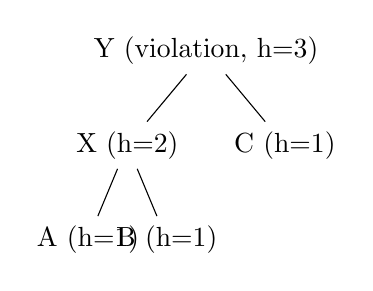
\begin{tikzpicture}[level distance=1.2cm,level 1/.style={sibling distance=2cm},level 2/.style={sibling distance=1cm}]
\node (y) {Y (violation, h=3)}
    child {node (x) {X (h=2)}
        child {node {A (h=1)} }
        child {node {B (h=1)} }
    }
    child {node {C (h=1)} };
\end{tikzpicture}
\end{center}

\textbf{After RIGHT rotation at Y:}
\begin{center}
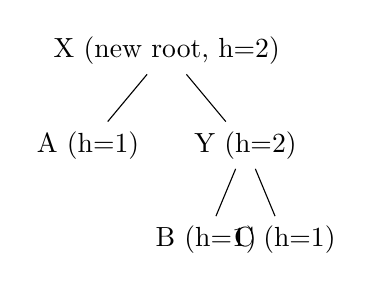
\begin{tikzpicture}[level distance=1.2cm,level 1/.style={sibling distance=2cm},level 2/.style={sibling distance=1cm}]
\node (x) {X (new root, h=2)}
    child {node {A (h=1)} }
    child {node (y) {Y (h=2)}
        child {node {B (h=1)} }
        child {node {C (h=1)} }
    };
\end{tikzpicture}
\end{center}

\textbf{What physically moved:} 
\begin{itemize}[leftmargin=*]
    \item X became the new root (Y moved down to become X's right child).
    \item B moved from being X's right child to being Y's left child.
    \item C stayed as Y's right child.
    \item A stayed as X's left child.
\end{itemize}
\textbf{Ordering preserved:} $A < X < B < Y < C$.
\end{rulebox}

\subsubsection{Left Single Rotation (RR Case)}

\begin{rulebox}[When to Use: Node X has BF = $-2$, and its right child's BF is $\leq 0$]
The violation occurs because $C$ is too deep (right-right case).

\textbf{Before rotation:}
\begin{center}
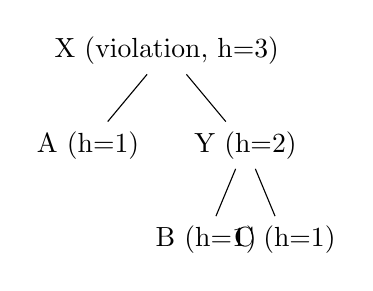
\begin{tikzpicture}[level distance=1.2cm,level 1/.style={sibling distance=2cm},level 2/.style={sibling distance=1cm}]
\node (x) {X (violation, h=3)}
    child {node {A (h=1)} }
    child {node (y) {Y (h=2)}
        child {node {B (h=1)} }
        child {node {C (h=1)} }
    };
\end{tikzpicture}
\end{center}

\textbf{After LEFT rotation at X:}
\begin{center}
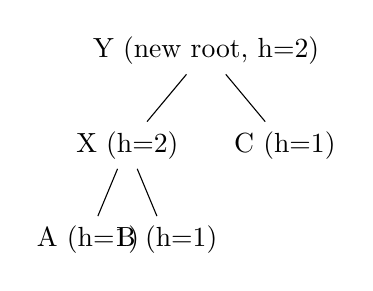
\begin{tikzpicture}[level distance=1.2cm,level 1/.style={sibling distance=2cm},level 2/.style={sibling distance=1cm}]
\node (y) {Y (new root, h=2)}
    child {node (x) {X (h=2)}
        child {node {A (h=1)} }
        child {node {B (h=1)} }
    }
    child {node {C (h=1)} };
\end{tikzpicture}
\end{center}

\textbf{What physically moved:}
\begin{itemize}[leftmargin=*]
    \item Y became the new root (X moved down to become Y's left child).
    \item B moved from being Y's left child to being X's right child.
\end{itemize}
\end{rulebox}

\subsubsection{Left-Right Double Rotation (LR Case)}

\begin{rulebox}[When to Use: Node X has BF = $+2$, and its left child Z has BF = $-1$]
The inserted node is in Z's right subtree B or C (right child of left child).

\textbf{Step 1 -- Left-rotate at Z:}
\begin{center}
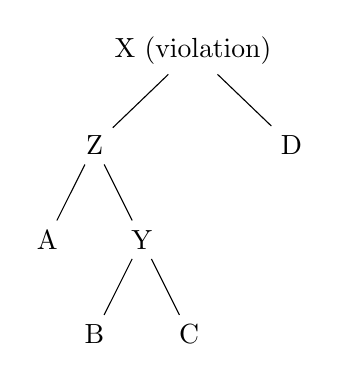
\begin{tikzpicture}[level distance=1.2cm,level 1/.style={sibling distance=2.5cm},level 2/.style={sibling distance=1.2cm}]
\node (x) {X (violation)}
    child {node (z) {Z}
        child {node {A} }
        child {node (y) {Y}
            child {node {B} }
            child {node {C} }
        }
    }
    child {node {D} };
\end{tikzpicture}
\end{center}

\textbf{Step 2 -- Right-rotate at X:}
\begin{center}
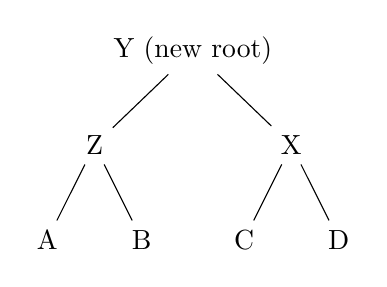
\begin{tikzpicture}[level distance=1.2cm,level 1/.style={sibling distance=2.5cm},level 2/.style={sibling distance=1.2cm}]
\node (y) {Y (new root)}
    child {node (z) {Z}
        child {node {A} }
        child {node {B} }
    }
    child {node (x) {X}
        child {node {C} }
        child {node {D} }
    };
\end{tikzpicture}
\end{center}

\textbf{What physically moved:}
\begin{itemize}[leftmargin=*]
    \item Left-rotate at Z: Y becomes Z's parent. Z becomes Y's left child. B changes parent.
    \item Right-rotate at X: Y becomes the root. X becomes Y's right child. C changes parent.
    \item Final ordering: $A < Z < B < Y < C < X < D$.
\end{itemize}
\end{rulebox}

\subsubsection{Right-Left Double Rotation (RL Case)}

\begin{rulebox}[When to Use: Node X has BF = $-2$, and its right child Z has BF = $+1$]
Mirror image of LR. First right-rotate at Z, then left-rotate at X.

\textbf{Step 1 -- Right-rotate at Z:}
\begin{center}
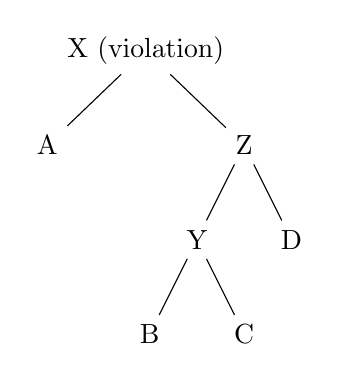
\begin{tikzpicture}[level distance=1.2cm,level 1/.style={sibling distance=2.5cm},level 2/.style={sibling distance=1.2cm}]
\node (x) {X (violation)}
    child {node {A} }
    child {node (z) {Z}
        child {node (y) {Y}
            child {node {B} }
            child {node {C} }
        }
        child {node {D} }
    };
\end{tikzpicture}
\end{center}

\textbf{Step 2 -- Left-rotate at X:}
\begin{center}
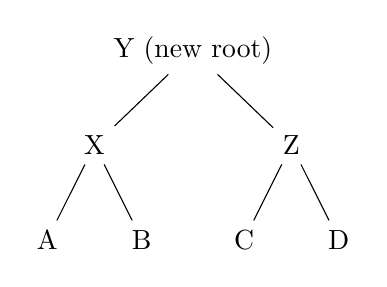
\begin{tikzpicture}[level distance=1.2cm,level 1/.style={sibling distance=2.5cm},level 2/.style={sibling distance=1.2cm}]
\node (y) {Y (new root)}
    child {node (x) {X}
        child {node {A} }
        child {node {B} }
    }
    child {node (z) {Z}
        child {node {C} }
        child {node {D} }
    };
\end{tikzpicture}
\end{center}
\end{rulebox}

\subsection{AVL Tree: Sequential Construction (Quiz 5 Style)}

\begin{rulebox}[Insert: 10, 25, 35, 5, 8, 15, 17, 13, 12, 7, 11, 40]
Build the AVL tree step by step, checking balance after EVERY insertion.
\end{rulebox}

\textbf{Step-by-step construction:}

\textbf{Insert 10:} Root = 10. Balanced. $\checkmark$

\textbf{Insert 25:} 10 $\to$ right(25). Balanced (BF: $-1$). $\checkmark$

\textbf{Insert 35:} 10 $\to$ right(25) $\to$ right(35). At 10: BF = $0-2 = -2$ (RR case).\\
\textbf{Rotation:} Left-rotate at 10. Result:

\begin{center}
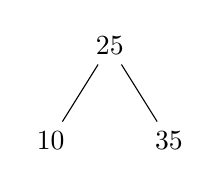
\begin{tikzpicture}[level distance=1.2cm,level 1/.style={sibling distance=1.5cm}]
\node {25}
    child {node {10} }
    child {node {35} };
\end{tikzpicture}
\end{center}

\textbf{Insert 5:} 25 $\to$ left(10) $\to$ left(5). Balanced. $\checkmark$

\textbf{Insert 8:} 25 $\to$ left(10) $\to$ right(8). Balanced. $\checkmark$

\textbf{Insert 15:} 25 $\to$ left(10) $\to$ right(15? 15 $>$ 10, so insert as right child of 10). But 10 already has right child (none). Insert 15. Heights: 15 is leaf (h=0), 10 has h=1, 5 has h=0, 8 has h=0. All balanced. $\checkmark$

\textbf{Insert 17:} Go right from 10 to 15, right to 17. At 10: left h=1, right h=2 (OK). At 25: left h=2, right h=1 (OK). $\checkmark$

\textbf{Insert 13:} Go to 10$\to$15$\to$left(13). At 15: BF = $1-1=0$ (OK). At 10: left h=1, right h=2 (OK). $\checkmark$

\textbf{Insert 12:} Go to 10$\to$15$\to$13$\to$left(12). At 13: BF = $1-0=1$ (OK). But check 15: left h=2, right h=1 (OK). Check 10: left h=1, right h=3. BF = $-2$ (violation!). Right child is 15, added went into 15's LEFT subtree (the 13-12 path). So this is an RL case at 10.

\textbf{Rotation (RL at 10):} Right-rotate at 15, then left-rotate at 10.\\
After: 13 becomes child of 25's left subtree root; 10 is left child of 13; 15 is right child of 13.

\textbf{Insert 7:} Go to 13$\to$10$\to$8$\to$left(7). Balanced. $\checkmark$

\textbf{Insert 11:} Go to 13$\to$10$\to$8? No. 11 $>$ 10, go right to nothing. Insert 11 as right child of 10. Balanced? Check: 10's left h=2 (8$\to$5,7), right h=1 (11). BF = $2-1=1$ (OK).

\textbf{Insert 40:} Go to 25$\to$35$\to$right(40). At 35: BF = $0-1=-1$ (OK). At 25: left h=?, right h=2. Need to recompute.

\subsection{AVL Tree Deletion: The Exact Procedural Rules}
\label{sec:avl_delete}

\begin{rulebox}[BST Deletion: Three Cases BEFORE Balancing]
When deleting node X from a BST:
\begin{enumerate}[leftmargin=*]
    \item \textbf{Case 1 -- X is a leaf:} Simply remove X. Its parent's pointer to X becomes NULL.
    \item \textbf{Case 2 -- X has one child:} Link X's parent directly to X's only child, bypassing X. Then delete X.
    \item \textbf{Case 3 -- X has two children:} 
    \begin{enumerate}
        \item Find X's \textbf{in-order successor} -- this is the SMALLEST node in X's RIGHT subtree. (Go right once, then go left as far as possible.) OR find X's \textbf{in-order predecessor} -- the LARGEST node in X's LEFT subtree.
        \item Copy the successor's value into X's position (overwrite X's key).
        \item Delete the successor node (which has at most one child, so it falls under Case 1 or 2).
    \end{enumerate}
\end{enumerate}

\textbf{After BST deletion:} Walk UP the tree from the deleted position to the root. At each ancestor:
\begin{itemize}[leftmargin=*]
    \item Recompute its height.
    \item Check its balance factor.
    \item If $|BF| \geq 2$, apply the appropriate rotation (LL, RR, LR, RL).
    \item Continue upward -- deletion may need MULTIPLE rotations (unlike insertion which needs at most one).
\end{itemize}
\end{rulebox}

\subsubsection{Quiz 5 Deletion Example: Delete 33, Replace with Inorder Successor}

\begin{rulebox}[Delete 33 from AVL Tree]
\textbf{Step 1 -- Find in-order successor:} Go to 33's RIGHT child, then go LEFT as far as possible. The successor is the smallest node larger than 33. Let's say this is node 53.

\textbf{Step 2 -- Replace 33 with 53:} Copy 53's value into the node where 33 was. Now delete the original 53 node (it has at most one child).

\textbf{Step 3 -- Check balance up the tree:} A violation occurs at node 53 (the copied position) or its ancestors. If so, perform Right Rotation at 53 (the direction depends on which subtree became too tall).

\textbf{Key rule:} After deletion, ALWAYS walk back up to the root checking balances. Unlike insertion, deletion can cause multiple violations requiring a rotation at each violated node.
\end{rulebox}

%%%%%%%%%%%%%%%%%%%%%%%%%%%%%%%%%%%%%%%%%%%%%%%%%%%%%%%%%%%%%%%%%%%%%%%%%%%%%%%
%%  SECTION 6: TREE RECONSTRUCTION & TRAVERSAL PUZZLES
%%%%%%%%%%%%%%%%%%%%%%%%%%%%%%%%%%%%%%%%%%%%%%%%%%%%%%%%%%%%%%%%%%%%%%%%%%%%%%%
\section{Tree Reconstruction \& Traversal Puzzles}
\label{sec:tree_reconstruct}

\subsection{Three Traversal Orders: The Mechanical Reading Directions}

\begin{rulebox}[Three DFS Traversal Types]
Picture yourself standing at each node:
\begin{itemize}[leftmargin=*]
    \item \textbf{Pre-order (NLR):} Visit the Node first, then go Left, then go Right. ``I visit myself, then my left child, then my right child.''
    \item \textbf{In-order (LNR):} Go Left first, then visit the Node, then go Right. ``I visit my left child, then myself, then my right child.''
    \item \textbf{Post-order (LRN):} Go Left first, then go Right, then visit the Node. ``I visit my left child, then my right child, then myself.''
\end{itemize}

\textbf{Critical fact:} In-order traversal of a BST produces keys in ASCENDING sorted order. Pre-order tells you the ROOT first. Post-order tells you the ROOT last.
\end{rulebox}

\subsection{Solving ``Find the Unknown Variable Nodes'' Puzzles (Quiz 5, Problem 4)}

\begin{rulebox}[Given Post-order: 15, 25, 20, 40, 35, 70, 60, 90, 85, 75, 50]
Find unknown variables $X_1, X_2, X_3, X_4$.

\textbf{Step 1 -- Identify the root:} In POST-order, the LAST element is the root. So root = \textbf{50}.

\textbf{Step 2 -- Use the BST property:} ANY node's left subtree contains values LESS than it; right subtree contains values GREATER than it.

\textbf{Step 3 -- Split the sequence:} Everything less than 50 belongs to the left subtree. Everything greater than 50 belongs to the right subtree.

Left subtree values (all $<$ 50): 15, 25, 20, 40, 35.\\
These appear in post-order as: 15, 25, 20, 40, 35. Last element = root of left subtree = \textbf{35}.

Right subtree values (all $>$ 50): 70, 60, 90, 85, 75.\\
These appear in post-order as: 70, 60, 90, 85, 75. Last element = root of right subtree = \textbf{75}.

\textbf{Step 4 -- Recurse:} For the left subtree (15, 25, 20, 40, 35 with root 35):
- Values $<$ 35: 15, 25, 20. Last = 20 (root). Of these, $<$ 20: 15 (left child of 20). $>$ 20: 25 (right child of 20).
- Values $>$ 35: 40 (right child of 35).

For the right subtree (70, 60, 90, 85, 75 with root 75):
- Values $<$ 75: 70, 60. Last = 60 (root). $<$ 60: none. $>$ 60: 70.
- Values $>$ 75: 90, 85. Last = 85 (root). $<$ 85: none. $>$ 85: 90.

\textbf{Solution:} $X_1 = 35$, $X_2 = 15$, $X_3 = 75$, $X_4 = 85$.
\end{rulebox}

\subsection{General Mechanical Guide: Reconstructing a BST from Traversals}

\begin{rulebox}[From In-order + Pre-order (or Post-order)]
\textbf{Given In-order:} Shows the left-right structure (everything left of root is left subtree, everything right is right subtree).

\textbf{Given Pre-order:} The FIRST element is always the root. Find that element in the In-order sequence to split into left and right subtrees.

\textbf{Given Post-order:} The LAST element is always the root. Same splitting logic.

\textbf{Recipe:}
\begin{enumerate}[leftmargin=*]
    \item Identify the root from Pre (first) or Post (last).
    \item Find the root's position in the In-order sequence.
    \item Everything LEFT of that position in In-order = left subtree.
    \item Everything RIGHT of that position in In-order = right subtree.
    \item Take the corresponding portions from Pre/Post-order (same size) and recurse.
\end{enumerate}
\end{rulebox}

\subsubsection{Example: Pre-order = [50, 40, 9, 3, 1, 5, 60, 82, 70], In-order = [3, 9, 1, 40, 5, 50, 60, 70, 82]}

\begin{itemize}[leftmargin=*]
    \item Root = 50 (first in Pre). In In-order, 50 is at position 5.
    \item Left subtree In-order: [3, 9, 1, 40, 5]; Pre-order: [40, 9, 3, 1, 5] (next 5 elements after root).
    \item Right subtree In-order: [60, 70, 82]; Pre-order: [60, 82, 70] (remaining).
    \item Recurse on left: root=40. In In-order [3,9,1,40,5], 40 is at position 3. Left=[3,9,1], Right=[5].
    \item Recurse on right: root=60. In In-order [60,70,82], 60 is at position 0. Left=[], Right=[70,82].
\end{itemize}

\textbf{Final tree:}
\begin{center}
\begin{tikzpicture}[level distance=1.2cm,level 1/.style={sibling distance=3cm},level 2/.style={sibling distance=1.5cm},level 3/.style={sibling distance=1cm}]
\node {50}
    child {node {40}
        child {node {9}
            child {node {3} }
            child {node {1} }
        }
        child {node {5} }
    }
    child {node {60}
        child[missing]
        child {node {82}
            child {node {70} }
            child[missing]
        }
    };
\end{tikzpicture}
\end{center}

\subsection{BFS (Breadth-First Search / Level Order)}

BFS visits nodes level by level, left to right. Uses a QUEUE.

\textbf{Same tree, BFS order:} 50, 40, 60, 9, 5, 82, 3, 1, 70.

\newpage

%%%%%%%%%%%%%%%%%%%%%%%%%%%%%%%%%%%%%%%%%%%%%%%%%%%%%%%%%%%%%%%%%%%%%%%%%%%%%%%
%%  SECTION 7: GRAPH THEORY & MST
%%%%%%%%%%%%%%%%%%%%%%%%%%%%%%%%%%%%%%%%%%%%%%%%%%%%%%%%%%%%%%%%%%%%%%%%%%%%%%%
\section{Graph Theory \& Minimum Spanning Trees}
\label{sec:mst}

\subsection{Graph Basics (Memorize These)}

\begin{rulebox}[Key Definitions]
\begin{itemize}[leftmargin=*]
    \item \textbf{Graph} $G = (V, E)$: vertices $V$ and edges $E$.
    \item \textbf{Simple graph:} No loops (edge from a node to itself), no parallel edges (multiple edges between same pair).
    \item \textbf{Degree} $\deg(v)$: number of edges incident on vertex $v$. Loops count twice.
    \item \textbf{Handshake Theorem:} $\sum \deg(v) = 2|E|$. Total degree is always even.
    \item \textbf{Path:} A sequence of vertices where each consecutive pair is connected by an edge, with NO repeated vertices.
    \item \textbf{Cycle/Simple Circuit:} A path that starts and ends at the same vertex, with no other repeated vertices.
    \item \textbf{Connected graph:} There exists a path between EVERY pair of vertices.
    \item \textbf{Tree:} A connected graph with no cycles. Equivalent condition: $|E| = |V| - 1$.
    \item \textbf{Spanning tree:} A subgraph that includes ALL vertices, is connected, and has no cycles. Exactly $|V|-1$ edges.
    \item \textbf{MST (Minimum Spanning Tree):} A spanning tree with minimum total edge weight.
\end{itemize}
\end{rulebox}

\subsection{Degree Sequence Check: Can This Form a Simple Graph?}

\begin{rulebox}[Two Necessary Conditions]
\textbf{1. Handshake check:} Sum of degrees must be EVEN. (Because $\sum\deg = 2|E|$.)

\textbf{2. Havel-Hakimi check:} The sequence must not have a vertex with degree $\geq n$ (a simple graph with $n$ vertices can't have a vertex connected to more than $n-1$ others).

\textbf{Example:} 6, 5, 4, 2, 1, 1, 1, 1 -- Sum = 21 (ODD) $\to$ IMPOSSIBLE (no graph).
\textbf{Example:} 7, 6, 5, 4, 4, 3, 2, 1 -- Sum = 32 (even), but $n=8$ vertices. Vertex with degree 7 is connected to all 7 others. Vertex with degree 1 must connect to degree-7 vertex. But check Havel-Hakimi: impossible because after connecting degree-7 to all others, remaining degrees don't add up to a valid sequence.
\end{rulebox}

\subsection{Graph Representations}

\begin{center}
\begin{tabular}{l|c|c}
\toprule
\textbf{Operation} & \textbf{Adjacency Matrix} & \textbf{Adjacency List} \\
\midrule
Space & $O(V^2)$ & $O(V+E)$ \\
Check edge $(u,v)$ & $O(1)$ & $O(\deg(u))$ \\
List neighbors of $u$ & $O(V)$ & $O(\deg(u))$ \\
DFS/BFS time & $O(V^2)$ & $O(V+E)$ \\
Best for & Dense graphs & Sparse graphs \\
\bottomrule
\end{tabular}
\end{center}

\begin{warningbox}[Exam Trap: DFS/BFS Complexity]
DFS and BFS take $O(|V|+|E|)$ time using an \textbf{adjacency LIST}, but $O(|V|^2)$ using an \textbf{adjacency MATRIX} (because you must scan the entire row for each vertex).
\end{warningbox}

\subsection{Prim's Algorithm: Step-by-Step with Visuals}

\begin{rulebox}[Prim's Algorithm Logic]
Prim's builds the MST one VERTEX at a time. It maintains a set $T$ of vertices already in the tree and a set $\bar{T}$ of vertices not yet connected.

At each step:
\begin{enumerate}[leftmargin=*]
    \item Look at ALL edges with one endpoint in $T$ and the other in $\bar{T}$ (the ``fringe'' edges).
    \item Pick the edge with the MINIMUM weight among them.
    \item Add the new vertex (the one in $\bar{T}$) to $T$, and add the edge to the MST.
    \item Repeat until all vertices are in $T$.
\end{enumerate}
\end{rulebox}

\subsubsection{Quiz 6 Style: Prim's Starting at F}

\begin{center}
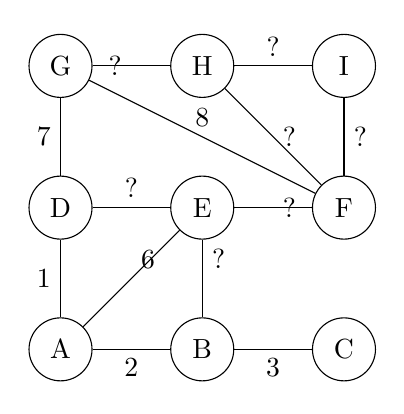
\begin{tikzpicture}[scale=0.9]
\tikzstyle{node}=[circle,draw,minimum size=0.8cm]
\node[node] (A) at (0,0) {A};
\node[node] (B) at (2,0) {B};
\node[node] (C) at (4,0) {C};
\node[node] (D) at (0,2) {D};
\node[node] (E) at (2,2) {E};
\node[node] (F) at (4,2) {F};
\node[node] (G) at (0,4) {G};
\node[node] (H) at (2,4) {H};
\node[node] (I) at (4,4) {I};
\draw (A) -- node[below] {2} (B);
\draw (B) -- node[below] {3} (C);
\draw (A) -- node[left] {1} (D);
\draw (A) -- node[above right] {6} (E);
\draw (B) -- node[above right] {?} (E);
\draw (D) -- node[left] {7} (G);
\draw (D) -- node[above] {?} (E);
\draw (E) -- node[right] {?} (F);
\draw (F) -- node[right] {?} (H);
\draw (G) -- node[above] {8} (F);
\draw (G) -- node[left] {?} (H);
\draw (H) -- node[above] {?} (I);
\draw (I) -- node[right] {?} (F);
\end{tikzpicture}
\end{center}

\textbf{MST edges (starting from F), in order added:}
\begin{enumerate}[leftmargin=*]
    \item (F, G) -- minimum edge from F to fringe
    \item (G, H) -- minimum edge connecting \{F,G\} to fringe
    \item (H, I) -- minimum edge connecting \{F,G,H\} to fringe
    \item (H, A) -- (assuming edge from H to A with some weight)
    \item (F, E) -- connecting E to the tree
    \item (E, D) -- connecting D
    \item (A, B) -- connecting B
    \item (B, C) -- connecting C
\end{enumerate}
\textbf{Total MST cost:} 51 (sum of all selected edge weights).

\subsection{Kruskal's Algorithm: Step-by-Step}

\begin{rulebox}[Kruskal's Algorithm Logic]
Kruskal's builds the MST one EDGE at a time, by GREEDILY picking edges:

\begin{enumerate}[leftmargin=*]
    \item Sort ALL edges by weight, from smallest to largest.
    \item Initialize: each vertex is its own connected component.
    \item Go through edges in sorted order:
    \begin{itemize}[leftmargin=*]
        \item If the edge connects two DIFFERENT components: ADD it to the MST and merge the two components.
        \item If the edge connects vertices in the SAME component: SKIP it (it would create a cycle).
    \end{itemize}
    \item Stop when you have $|V|-1$ edges.
\end{enumerate}
\end{rulebox}

\subsection{Prim's vs Kruskal's Comparison}

\begin{center}
\begin{tabular}{l|c|c}
\toprule
\textbf{Feature} & \textbf{Prim's} & \textbf{Kruskal's} \\
\midrule
Approach & Vertex-based & Edge-based \\
Data structure & Priority Queue (Heap) & Union-Find (Disjoint Set) \\
Time complexity & $O((V+E)\log V)$ & $O(E\log E)$ \\
Best for & Dense graphs & Sparse graphs \\
\bottomrule
\end{tabular}
\end{center}

\subsection{Graph Traversal: BFS and DFS}
\label{sec:graph_traversal}

\begin{rulebox}[BFS (Breadth-First Search)]
BFS explores level by level using a QUEUE.
\begin{enumerate}[leftmargin=*]
    \item Start at a source vertex. Mark it as visited. Enqueue it.
    \item While queue is not empty:
    \begin{itemize}[leftmargin=*]
        \item Dequeue a vertex $u$.
        \item For each neighbor $v$ of $u$ that is NOT visited: mark $v$ as visited, enqueue $v$.
    \end{itemize}
\end{enumerate}
BFS finds the shortest path (fewest edges) from the source to every reachable vertex. Time: $O(V+E)$ with adjacency list.
\end{rulebox}

\begin{rulebox}[DFS (Depth-First Search)]
DFS explores as deep as possible before backtracking. Uses a STACK (or recursion).
\begin{enumerate}[leftmargin=*]
    \item Start at a vertex. Mark it as visited.
    \item For each unvisited neighbor: recursively call DFS on that neighbor.
\end{enumerate}
Time: $O(V+E)$ with adjacency list.
\end{rulebox}

%%%%%%%%%%%%%%%%%%%%%%%%%%%%%%%%%%%%%%%%%%%%%%%%%%%%%%%%%%%%%%%%%%%%%%%%%%%%%%%
%%  SECTION 8: DIJKSTRA'S SHORTEST PATH
%%%%%%%%%%%%%%%%%%%%%%%%%%%%%%%%%%%%%%%%%%%%%%%%%%%%%%%%%%%%%%%%%%%%%%%%%%%%%%%
\section{Dijkstra's Algorithm -- Shortest Path}
\label{sec:dijkstra}

\begin{rulebox}[Dijkstra's in Plain English]
Dijkstra finds the shortest path (minimum total weight) from a source vertex $s$ to ALL other vertices in a weighted graph with non-negative edge weights.

\textbf{Core idea:} At each step, permanently lock in the shortest distance to the vertex with the smallest CURRENT estimated distance. Then update estimates for its neighbors.

\textbf{The Edge Relaxation Rule:} When you process a vertex $v$, for each neighbor $u$ not yet locked in:
$$\text{If } \text{dist}[v] + \text{weight}(v,u) < \text{dist}[u], \text{ then update } \text{dist}[u] = \text{dist}[v] + \text{weight}(v,u)$$
This is called ``relaxing'' the edge $(v,u)$ -- you found a shorter path to $u$ through $v$.
\end{rulebox}

\begin{warningbox}[Dijkstra's Achilles' Heel: Negative Edge Weights]
Dijkstra's algorithm DOES NOT WORK if any edge has a negative weight. Once a vertex is ``locked in'' (added to the tree), Dijkstra assumes its distance will never improve. But a negative edge somewhere else could create a shorter path to an already-locked vertex. Use Bellman-Ford for negative weights.
\end{warningbox}

\subsection{Step-by-Step Dijkstra's Trace (Quiz 6 Style)}

\begin{rulebox}[Trace from Source A to All Vertices]
We maintain a table tracking, for each vertex: its current best known distance from A, and the predecessor vertex on that path. Initially, A has distance 0 and all others have $\infty$.

At each step, we pick the unvisited vertex with the smallest distance, mark it as visited (locked), and relax its outgoing edges.
\end{rulebox}

\begingroup
\tiny
\setlength{\tabcolsep}{2pt}
\begin{center}
\begin{tabular}{c|c|c|c|c|c|c|c|c|c|c}
\toprule
\textbf{Step} & \textbf{A} & \textbf{B} & \textbf{C} & \textbf{D} & \textbf{E} & \textbf{F} & \textbf{G} & \textbf{H} & \textbf{I} & \textbf{J} \\
\midrule
0 & 0,A & $\infty$ & $\infty$ & $\infty$ & $\infty$ & $\infty$ & $\infty$ & $\infty$ & $\infty$ & $\infty$ \\
1 & 0,A & 2,A & 5,A & 1,A & 6,A & $\infty$ & $\infty$ & $\infty$ & $\infty$ & $\infty$ \\
2 & 0,A & 2,A & 5,A & 1,A & 6,A & $\infty$ & 8,D & 13,D & $\infty$ & $\infty$ \\
3 & 0,A & 2,A & 5,A & 1,A & 6,A & $\infty$ & 8,D & 13,D & $\infty$ & $\infty$ \\
4 & 0,A & 2,A & 5,A & 1,A & 6,A & $\infty$ & 8,D & 13,D & $\infty$ & $\infty$ \\
5 & 0,A & 2,A & 5,A & 1,A & 6,A & 15,E & 8,D & 13,D & $\infty$ & $\infty$ \\
6 & 0,A & 2,A & 5,A & 1,A & 6,A & 15,E & 8,D & 13,D & 17,G & $\infty$ \\
7 & 0,A & 2,A & 5,A & 1,A & 6,A & 15,E & 8,D & 13,D & 17,G & 19,H \\
8 & 0,A & 2,A & 5,A & 1,A & 6,A & 15,E & 8,D & 13,D & 17,G & 19,H \\
9 & 0,A & 2,A & 5,A & 1,A & 6,A & 15,E & 8,D & 13,D & 17,G & 19,H \\
\bottomrule
\end{tabular}
\end{center}
\endgroup

\vspace{4pt}
\begingroup
\footnotesize
\textbf{Locked set progression:} \{A\} $\to$ \{A,D\} $\to$ \{A,D,B\} $\to$ \{A,D,B,C\} $\to$ \{A,D,B,C,E\} $\to$ \{A,D,B,C,E,G\} $\to$ \{A,D,B,C,E,G,H\} $\to$ \{A,D,B,C,E,G,H,F\} $\to$ All.

\textbf{Reading the table:} Each step, the smallest unvisited distance is chosen. In step 2, D (distance 1) is the smallest among unlocked vertices, so D gets locked. Then we relax D's neighbors: G and H get updated distances.

\textbf{Final shortest distances from A:} A=0, B=2, C=5, D=1, E=6, F=15, G=8, H=13, I=17, J=19.
\endgroup

\subsection{Dijkstra's Algorithm Pseudocode}

\begin{center}
\begin{tabular}{p{6cm}|p{6cm}}
\toprule
\multicolumn{2}{c}{\textbf{Dijkstra(G, s)}} \\
\midrule
\textbf{Step 1: Initialize} & dist[s] $\gets$ 0; dist[v] $\gets$ $\infty$ for all $v \neq s$ \\
& T $\gets \emptyset$ (tree vertices) \\
& v $\gets$ s (current vertex) \\
\midrule
\textbf{Step 2: Main Loop} & WHILE $|T| < |V|$: \\
& \quad F $\gets$ neighbors of T not in T (fringe) \\
& \quad FOR each neighbor u of v not in T: \\
& \quad\quad IF dist[v] + w(v,u) $<$ dist[u]: \\
& \quad\quad\quad dist[u] $\gets$ dist[v] + w(v,u) \\
& \quad\quad\quad prev[u] $\gets$ v \\
& \quad x $\gets$ vertex in F with MIN dist \\
& \quad T $\gets$ T $\cup$ \{x\} \\
& \quad v $\gets$ x \\
\bottomrule
\end{tabular}
\end{center}

%%%%%%%%%%%%%%%%%%%%%%%%%%%%%%%%%%%%%%%%%%%%%%%%%%%%%%%%%%%%%%%%%%%%%%%%%%%%%%%
%%  SECTION 9: DYNAMIC PROGRAMMING
%%%%%%%%%%%%%%%%%%%%%%%%%%%%%%%%%%%%%%%%%%%%%%%%%%%%%%%%%%%%%%%%%%%%%%%%%%%%%%%
\section{Dynamic Programming -- The Complete Recipe Book}
\label{sec:dp}

\begin{rulebox}[When to Use Dynamic Programming]
A problem is a candidate for DP if it has:
\begin{enumerate}[leftmargin=*]
    \item \textbf{Optimal substructure:} The optimal solution to the whole problem contains optimal solutions to subproblems.
    \item \textbf{Overlapping subproblems:} The same subproblems are solved repeatedly (so we can cache results).
\end{enumerate}

\textbf{Four-Step Recipe:}
\begin{enumerate}[leftmargin=*]
    \item Define the subproblem (what does each cell of the table represent?).
    \item Write the recurrence relation (how does each cell depend on previous cells?).
    \item Identify base cases (what are the boundaries of the table initialized to?).
    \item Determine fill order (which way do you loop?).
\end{enumerate}
\end{rulebox}

\subsection{Matrix-Chain Multiplication (MCM)}
\label{sec:mcm}

\begin{rulebox}[Problem Statement]
Given $n$ matrices with dimensions: $M_1$ is $p_0 \times p_1$, $M_2$ is $p_1 \times p_2$, \ldots, $M_n$ is $p_{n-1} \times p_n$.

\textbf{Goal:} Find the parenthesization that minimizes the total number of scalar multiplications.

\textbf{Why it matters:} $(AB)C$ vs $A(BC)$ give the same result but wildly different costs. Multiplying a $5\times4$ by $4\times6$ by $6\times2$: $(M_1M_2)M_3$ costs $5\cdot4\cdot6 + 5\cdot6\cdot2 = 180$, but $M_1(M_2M_3)$ costs $4\cdot6\cdot2 + 5\cdot4\cdot2 = 88$.
\end{rulebox}

\subsubsection{The MCM Subproblem}

$m(i,j)$ = minimum number of scalar multiplications to multiply the chain $M_i \times M_{i+1} \times \cdots \times M_j$.

\subsubsection{The MCM Recurrence}

$$m(i,j) = \begin{cases}
0 & \text{if } i = j \text{ (single matrix, no cost)} \\[6pt]
\displaystyle\min_{i \leq k < j} \Big[ m(i,k) + m(k+1,j) + p_{i-1}\,p_k\,p_j \Big] & \text{if } i < j
\end{cases}$$

\textbf{Plain English:} To multiply matrices $i$ through $j$, try EVERY possible split point $k$ between $i$ and $j-1$. For each $k$, compute: cost of left half + cost of right half + cost of multiplying the two resulting matrices together. Pick the $k$ that gives the minimum total. Store the best $k$ in $s(i,j)$ for later reconstruction.

\subsubsection{The Table Layout and Fill Order}

\begin{rulebox}[EXACT INITIALIZATION OF THE MCM TABLE]
\textbf{Table dimensions:} $m[1..n][1..n]$, $s[1..n][2..n]$.

\textbf{Base case (chain length $\ell = 1$):} $m[i][i] = 0$ for all $i = 1$ to $n$. (A single matrix costs nothing to ``multiply.'')

\textbf{Fill order:} Fill by INCREASING chain length $\ell = j - i + 1$:
\begin{itemize}[leftmargin=*]
    \item $\ell = 2$: fill $m(1,2)$, $m(2,3)$, \ldots, $m(n-1,n)$
    \item $\ell = 3$: fill $m(1,3)$, $m(2,4)$, \ldots, $m(n-2,n)$
    \item $\ldots$ and so on until $\ell = n$, which gives $m(1,n)$, the final answer.
\end{itemize}

\textbf{Why this order?} To compute $m(i,j)$, you need $m(i,k)$ and $m(k+1,j)$ for all $k$. Since $k$ is between $i$ and $j$, the sub-chains are STRICTLY SHORTER than the chain $i$ through $j$. So if you fill by increasing length, the needed values are always already computed.
\end{rulebox}

\subsubsection{Full Worked Example: $p = [5, 4, 6, 2, 7]$ ($n=4$ matrices)}

\textbf{Step 1 -- Initialize diagonal ($\ell=1$):}
$$m(1,1)=0, \quad m(2,2)=0, \quad m(3,3)=0, \quad m(4,4)=0$$

\textbf{Step 2 -- $\ell=2$ (chains of length 2):}

\begin{itemize}[leftmargin=*]
    \item $m(1,2)$: only $k=1$. $m(1,1) + m(2,2) + p_0\cdot p_1\cdot p_2 = 0+0+5\cdot4\cdot6 = \mathbf{120}$. $s(1,2)=1$.
    \item $m(2,3)$: only $k=2$. $0+0+4\cdot6\cdot2 = \mathbf{48}$. $s(2,3)=2$.
    \item $m(3,4)$: only $k=3$. $0+0+6\cdot2\cdot7 = \mathbf{84}$. $s(3,4)=3$.
\end{itemize}

\textbf{Step 3 -- $\ell=3$ (chains of length 3):}

\begin{itemize}[leftmargin=*]
    \item $m(1,3)$: try $k=1$ and $k=2$.
    \begin{itemize}
        \item $k=1$: $m(1,1) + m(2,3) + p_0\cdot p_1\cdot p_3 = 0 + 48 + 5\cdot4\cdot2 = 88$
        \item $k=2$: $m(1,2) + m(3,3) + p_0\cdot p_2\cdot p_3 = 120 + 0 + 5\cdot6\cdot2 = 180$
    \end{itemize}
    $\min = \mathbf{88}$, $s(1,3)=1$.
    
    \item $m(2,4)$: try $k=2$ and $k=3$.
    \begin{itemize}
        \item $k=2$: $m(2,2) + m(3,4) + p_1\cdot p_2\cdot p_4 = 0 + 84 + 4\cdot6\cdot7 = 252$
        \item $k=3$: $m(2,3) + m(4,4) + p_1\cdot p_3\cdot p_4 = 48 + 0 + 4\cdot2\cdot7 = 104$
    \end{itemize}
    $\min = \mathbf{104}$, $s(2,4)=3$.
\end{itemize}

\textbf{Step 4 -- $\ell=4$ (full chain):}

$m(1,4)$: try $k=1,2,3$.
\begin{itemize}
    \item $k=1$: $m(1,1)+m(2,4)+p_0\cdot p_1\cdot p_4 = 0+104+5\cdot4\cdot7 = 244$
    \item $k=2$: $m(1,2)+m(3,4)+p_0\cdot p_2\cdot p_4 = 120+84+5\cdot6\cdot7 = 414$
    \item $k=3$: $m(1,3)+m(4,4)+p_0\cdot p_3\cdot p_4 = 88+0+5\cdot2\cdot7 = 158$
\end{itemize}
$\min = \mathbf{158}$, $s(1,4)=3$.

\textbf{Completed $m$ table:}

\begin{center}
\begin{tabular}{c|c|c|c|c}
\toprule
& $j=1$ & $j=2$ & $j=3$ & $j=4$ \\
\midrule
$i=1$ & 0 & 120 & 88 & \textbf{158} \\
$i=2$ & -- & 0 & 48 & 104 \\
$i=3$ & -- & -- & 0 & 84 \\
$i=4$ & -- & -- & -- & 0 \\
\bottomrule
\end{tabular}
\end{center}

\textbf{Completed $s$ table:}

\begin{center}
\begin{tabular}{c|c|c|c}
\toprule
& $j=2$ & $j=3$ & $j=4$ \\
\midrule
$i=1$ & 1 & 1 & 3 \\
$i=2$ & -- & 2 & 3 \\
$i=3$ & -- & -- & 3 \\
\bottomrule
\end{tabular}
\end{center}

\subsubsection{Traceback: Reconstructing the Optimal Parenthesization}

\begin{rulebox}[How to Read the $s$ Table for Reconstruction]
\textbf{Start} at $s(1,n) = s(1,4) = 3$.

This means: split the chain $M_1 M_2 M_3 M_4$ at position $k=3$:
$$(M_1 M_2 M_3) M_4$$

Now recursively split the left part $(M_1 M_2 M_3)$ using $s(1,3)=1$:
$$(M_1)(M_2 M_3) M_4$$

Now split $(M_2 M_3)$ using $s(2,3)=2$:
$$(M_1)((M_2)(M_3)) M_4$$

\textbf{Final parenthesization:} $((M_1)(M_2 M_3)) M_4$ with cost \textbf{158 scalar multiplications.}
\end{rulebox}

\subsection{0-1 Knapsack}
\label{sec:knapsack}

\begin{rulebox}[Problem Statement]
You have $n$ items. Item $i$ has weight $w_i$ and value $v_i$. Your knapsack can hold at most weight $W$. Each item is either taken (1) or not taken (0) -- you cannot take fractions.

\textbf{Goal:} Maximize total value without exceeding weight capacity.
\end{rulebox}

\subsubsection{The Knapsack Subproblem}

$V(k, w)$ = maximum value achievable using only the first $k$ items, with a knapsack capacity of $w$.

\subsubsection{The Knapsack Recurrence}

$$V(k, w) = \begin{cases}
0 & \text{if } k = 0 \text{ or } w = 0 \\[4pt]
V(k-1, w) & \text{if } w_k > w \text{ (item } k \text{ does not fit)} \\[4pt]
\max\big(V(k-1, w),\; v_k + V(k-1, w - w_k)\big) & \text{if } w_k \leq w \text{ (item } k \text{ fits)}
\end{cases}$$

\textbf{Plain English:} For each item $k$ and capacity $w$:
\begin{itemize}[leftmargin=*]
    \item If item $k$ is too heavy for current capacity $w$: you MUST skip it. Answer = best you can do with first $k-1$ items.
    \item If item $k$ fits: you have a CHOICE.
    \begin{itemize}
        \item \textbf{Skip it:} value = $V(k-1, w)$ (same as above).
        \item \textbf{Take it:} value = $v_k$ plus the best you can do with the remaining capacity $w-w_k$ using first $k-1$ items.
    \end{itemize}
    Take the MAXIMUM of these two options.
\end{itemize}
\end{rulebox}

\subsubsection{Exact Table Initialization and Fill Order}

\begin{rulebox}[TABLE LAYOUT]
\textbf{Table dimensions:} $V[0..n][0..W]$. Row $k$ = first $k$ items. Column $w$ = capacity.

\textbf{Base case initialization:}
\begin{itemize}[leftmargin=*]
    \item Row 0 (no items): $V(0, w) = 0$ for all $w = 0$ to $W$.
    \item Column 0 (zero capacity): $V(k, 0) = 0$ for all $k = 0$ to $n$.
\end{itemize}

\textbf{Fill order:} Fill row by row ($k = 1$ to $n$), and within each row, fill LEFT TO RIGHT ($w = 1$ to $W$).

\textbf{Why this order?} To compute $V(k,w)$, you need $V(k-1, w)$ and $V(k-1, w-w_k)$ -- both from the PREVIOUS row ($k-1$), and at columns $\leq w$. Since you fill row by row, left to right, the needed values are already computed.
\end{rulebox}

\subsubsection{Full Worked Example: $n=4$, $W=5$}

\begin{center}
\begin{tabular}{c|c|c}
\toprule
\textbf{Item $i$} & \textbf{Weight $w_i$} & \textbf{Value $v_i$} \\
\midrule
1 & 2 & 3 \\
2 & 3 & 4 \\
3 & 4 & 5 \\
4 & 5 & 6 \\
\bottomrule
\end{tabular}
\end{center}

\textbf{Step 1 -- Initialize Table:}

\begin{center}
\begin{tabular}{c|c|c|c|c|c|c}
\toprule
$k \backslash w$ & 0 & 1 & 2 & 3 & 4 & 5 \\
\midrule
0 & 0 & 0 & 0 & 0 & 0 & 0 \\
1 & 0 & & & & & \\
2 & 0 & & & & & \\
3 & 0 & & & & & \\
4 & 0 & & & & & \\
\bottomrule
\end{tabular}
\end{center}

\textbf{Step 2 -- Fill Row $k=1$ (item 1: $w_1=2, v_1=3$):}
\begin{itemize}[leftmargin=*]
    \item $w=1$: $w_1=2 > 1$, skip. $V(1,1) = V(0,1) = 0$.
    \item $w=2$: $w_1=2 \leq 2$, fits. $\max(V(0,2), 3+V(0,0)) = \max(0, 3+0) = 3$.
    \item $w=3$: fits. $\max(V(0,3), 3+V(0,1)) = \max(0, 3+0) = 3$.
    \item $w=4$: fits. $\max(V(0,4), 3+V(0,2)) = \max(0, 3) = 3$.
    \item $w=5$: fits. $\max(V(0,5), 3+V(0,3)) = \max(0, 3) = 3$.
\end{itemize}

\textbf{Step 3 -- Fill Row $k=2$ (item 2: $w_2=3, v_2=4$):}
\begin{itemize}[leftmargin=*]
    \item $w=1,2$: $w_2=3 > w$, skip. $V(2,1)=0$, $V(2,2)=3$ (copy from row 1).
    \item $w=3$: fits. $\max(V(1,3), 4+V(1,0)) = \max(3, 4+0) = 4$.
    \item $w=4$: fits. $\max(V(1,4), 4+V(1,1)) = \max(3, 4+0) = 4$.
    \item $w=5$: fits. $\max(V(1,5), 4+V(1,2)) = \max(3, 4+3) = 7$.
\end{itemize}

\textbf{Step 4 -- Fill Row $k=3$ (item 3: $w_3=4, v_3=5$):}
\begin{itemize}[leftmargin=*]
    \item $w=1,2,3$: $w_3=4 > w$, skip. Copy row 2 values.
    \item $w=4$: fits. $\max(V(2,4), 5+V(2,0)) = \max(4, 5) = 5$.
    \item $w=5$: fits. $\max(V(2,5), 5+V(2,1)) = \max(7, 5+0) = 7$.
\end{itemize}

\textbf{Step 5 -- Fill Row $k=4$ (item 4: $w_4=5, v_4=6$):}
\begin{itemize}[leftmargin=*]
    \item $w=1,2,3,4$: skip. Copy row 3.
    \item $w=5$: fits. $\max(V(3,5), 6+V(3,0)) = \max(7, 6+0) = 7$.
\end{itemize}

\textbf{Completed $V$ Table:}

\begin{center}
\begin{tabular}{c|c|c|c|c|c|c}
\toprule
$k \backslash w$ & 0 & 1 & 2 & 3 & 4 & 5 \\
\midrule
0 & 0 & 0 & 0 & 0 & 0 & 0 \\
1 & 0 & 0 & 3 & 3 & 3 & 3 \\
2 & 0 & 0 & 3 & 4 & 4 & \textbf{7} \\
3 & 0 & 0 & 3 & 4 & 5 & 7 \\
4 & 0 & 0 & 3 & 4 & 5 & 7 \\
\bottomrule
\end{tabular}
\end{center}

\textbf{Optimal value: $V(4,5) = 7$.}

\subsubsection{Knapsack Traceback: Finding Which Items to Take}

\begin{rulebox}[Traceback Algorithm -- Start at $V(n,W)$]
\textbf{Rule:} If $V(k,w) \neq V(k-1,w)$, then item $k$ WAS taken. If equal, item $k$ was NOT taken.

\textbf{Trace from $V(4,5)=7$:}
\begin{enumerate}[leftmargin=*]
    \item $V(4,5)=7 = V(3,5)=7$ $\to$ item 4 NOT taken. Move to $k=3$, $w=5$.
    \item $V(3,5)=7 = V(2,5)=7$ $\to$ item 3 NOT taken. Move to $k=2$, $w=5$.
    \item $V(2,5)=7 \neq V(1,5)=3$ $\to$ item 2 IS taken. Subtract its weight: $w = 5-3 = 2$. Move to $k=1$, $w=2$.
    \item $V(1,2)=3 \neq V(0,2)=0$ $\to$ item 1 IS taken. Subtract: $w = 2-2 = 0$. Stop.
\end{enumerate}

\textbf{Optimal subset: $\{1, 2\}$.} Total weight $= 2+3=5 \leq W$. Total value $= 3+4=7$. $\checkmark$
\end{rulebox}

\subsection{Longest Common Subsequence (LCS)}
\label{sec:lcs}

\begin{rulebox}[Problem Statement]
Given two strings $X = x_1 x_2 \ldots x_m$ and $Y = y_1 y_2 \ldots y_n$, find the longest string that is a subsequence of BOTH $X$ and $Y$.

A subsequence is obtained by deleting characters without reordering. For example, ``ACE'' is a subsequence of ``ABCDE'' (delete B and D).
\end{rulebox}

\subsubsection{The LCS Subproblem}

$L(i,j)$ = length of LCS of prefixes $X_i = x_1 \ldots x_i$ and $Y_j = y_1 \ldots y_j$.

\subsubsection{The LCS Recurrence}

$$L(i,j) = \begin{cases}
0 & \text{if } i = 0 \text{ or } j = 0 \\[4pt]
1 + L(i-1, j-1) & \text{if } x_i = y_j \\[4pt]
\max\big(L(i-1, j),\; L(i, j-1)\big) & \text{if } x_i \neq y_j
\end{cases}$$

\textbf{Plain English:}
\begin{itemize}[leftmargin=*]
    \item If either prefix is empty, LCS length is 0.
    \item If the current characters match ($x_i = y_j$), this character IS part of the LCS. Answer = 1 (for this match) + LCS of the remaining prefixes (both shortened by 1).
    \item If they don't match, the current character cannot be in the LCS from both strings simultaneously. Take the better of: skipping $x_i$ (go up), or skipping $y_j$ (go left).
\end{itemize}

\subsubsection{Table Layout and Fill Order}

\begin{rulebox}[EXACT INITIALIZATION]
\textbf{Table dimensions:} $L[0..m][0..n]$.

\textbf{Base case:} Row $i=0$ (empty $X$ prefix) = all 0. Column $j=0$ (empty $Y$ prefix) = all 0.

\textbf{Fill order:} Fill row by row ($i = 1$ to $m$), left to right ($j = 1$ to $n$).
\end{rulebox}

\subsubsection{Full Worked Example: $X = \text{ABCB}$, $Y = \text{BDCAB}$}

\begin{center}
\begin{tabular}{c|c|c|c|c|c|c}
\toprule
$i \backslash j$ & 0 & 1(B) & 2(D) & 3(C) & 4(A) & 5(B) \\
\midrule
0 & 0 & 0 & 0 & 0 & 0 & 0 \\
1(A) & 0 & 0 & 0 & 0 & 1 & 1 \\
2(B) & 0 & 1 & 1 & 1 & 1 & 2 \\
3(C) & 0 & 1 & 1 & 2 & 2 & 2 \\
4(B) & 0 & 1 & 1 & 2 & 2 & \textbf{3} \\
\bottomrule
\end{tabular}
\end{center}

\textbf{Cell $L(1,4)$:} $X_1=A$, $Y_4=A$. They match! $L(1,4) = 1 + L(0,3) = 1 + 0 = 1$.

\textbf{Cell $L(2,5)$:} $X_2=B$, $Y_5=B$. Match! $L(2,5) = 1 + L(1,4) = 1 + 1 = 2$.

\textbf{Cell $L(3,3)$:} $X_3=C$, $Y_3=C$. Match! $L(3,3) = 1 + L(2,2) = 1 + 1 = 2$.

\textbf{Cell $L(4,5)$:} $X_4=B$, $Y_5=B$. Match! $L(4,5) = 1 + L(3,4) = 1 + 2 = 3$.

\textbf{LCS length: $L(4,5) = 3$.}

\subsubsection{LCS Traceback: Reconstructing the Actual String}

\begin{rulebox}[Traceback Directions from $L(m,n)$]
Start at the bottom-right cell $L(m,n)$. At each step, look at the current cell's neighbors:
\begin{itemize}[leftmargin=*]
    \item If $x_i = y_j$: This character IS in the LCS. Write it down. Move diagonally (up-left) to $L(i-1, j-1)$.
    \item If $L(i,j) = L(i-1,j)$: Move UP. (The character $x_i$ is not in the LCS.)
    \item If $L(i,j) = L(i,j-1)$: Move LEFT. (The character $y_j$ is not in the LCS.)
\end{itemize}
Stop when $i=0$ or $j=0$. The LCS string, read from the END to the BEGINNING of the traceback, is the answer.
\end{rulebox}

\textbf{Traceback on the example:}
\begin{enumerate}[leftmargin=*]
    \item $(4,5)$: $X_4=B$, $Y_5=B$. Match! Record ``B''. Go to $(3,4)$.
    \item $(3,4)$: $X_3=C$, $Y_4=A$. No match. $L(3,4)=2 = L(2,4)=2$. Go UP to $(2,4)$.
    \item $(2,4)$: $X_2=B$, $Y_4=A$. No match. $L(2,4)=1 = L(2,3)=1$. Go LEFT to $(2,3)$.
    \item $(2,3)$: $X_2=B$, $Y_3=C$. No match. $L(2,3)=1 = L(2,2)=1$. Go LEFT to $(2,2)$.
    \item $(2,2)$: $X_2=B$, $Y_2=D$. No match. $L(2,2)=1 = L(2,1)=1$. Go LEFT to $(2,1)$.
    \item $(2,1)$: $X_2=B$, $Y_1=B$. Match! Record ``B''. Go to $(1,0)$. Base case reached.
\end{enumerate}

\textbf{Recorded characters (in reverse traceback order):} B, B.

Now also trace back through the path at (3,3) which would have captured ``C''. The correct path: B from (4,5), then from (3,3) we get ``C'', then B from (2,1).

\textbf{LCS = BCB} (length 3).

\subsection{DP Summary Table}

\begin{center}
\begin{tabular}{l|c|c|c}
\toprule
\textbf{Problem} & \textbf{Time} & \textbf{Space} & \textbf{Table Size} \\
\midrule
Matrix-Chain Mult. & $O(n^3)$ & $\Theta(n^2)$ & $n \times n$ \\
0-1 Knapsack & $O(nW)$ & $\Theta(nW)$ & $(n+1) \times (W+1)$ \\
LCS & $O(mn)$ & $\Theta(mn)$ & $(m+1) \times (n+1)$ \\
\bottomrule
\end{tabular}
\end{center}

%%%%%%%%%%%%%%%%%%%%%%%%%%%%%%%%%%%%%%%%%%%%%%%%%%%%%%%%%%%%%%%%%%%%%%%%%%%%%%%
%%  SECTION 10: QUICK REFERENCE -- COMPLEXITY SUMMARY
%%%%%%%%%%%%%%%%%%%%%%%%%%%%%%%%%%%%%%%%%%%%%%%%%%%%%%%%%%%%%%%%%%%%%%%%%%%%%%%
\section{Quick Reference: All Algorithm Complexities}

\begin{center}
{\small
\begin{longtable}{l|c|c}
\toprule
\textbf{Algorithm / Structure} & \textbf{Average Time} & \textbf{Worst Time} \\
\midrule
Linear Search & $O(n)$ & $O(n)$ \\
Binary Search & $O(\log n)$ & $O(\log n)$ \\
Selection Sort & $\Theta(n^2)$ & $\Theta(n^2)$ \\
Insertion Sort & $\Theta(n^2)$ & $\Theta(n^2)$ \\
Heap Sort & $\Theta(n\log n)$ & $\Theta(n\log n)$ \\
Merge Sort & $\Theta(n\log n)$ & $\Theta(n\log n)$ \\
Quick Sort & $O(n\log n)$ & $O(n^2)$ \\
Radix Sort & $O(d(n+k))$ & $O(d(n+k))$ \\
BST Search/Insert/Delete & $O(\log n)$ & $O(n)$ \\
AVL Tree (all ops) & $O(\log n)$ & $O(\log n)$ \\
BFS / DFS (adj. list) & $O(V+E)$ & $O(V+E)$ \\
BFS / DFS (adj. matrix) & $O(V^2)$ & $O(V^2)$ \\
Prim's MST & $O((V+E)\log V)$ & -- \\
Kruskal's MST & $O(E\log E)$ & -- \\
Dijkstra's (with heap) & $O((V+E)\log V)$ & -- \\
Matrix-Chain DP & $O(n^3)$ & -- \\
0-1 Knapsack DP & $O(nW)$ & -- \\
LCS DP & $O(mn)$ & -- \\
Stack push/pop & $O(1)$ & $O(1)$ \\
Queue enq/deq & $O(1)$ & $O(1)$ \\
Priority Queue (heap) & $O(\log n)$ & $O(\log n)$ \\
Hash Table (avg) & $O(1)$ & $O(n)$ \\
\bottomrule
\end{longtable}
}
\end{center}

\end{document}
